% !TeX root = ..\TGIII\main.tex




\documentclass[
	% -- opções da classe memoir --
	12pt,				% tamanho da fonte
	openright,			% capítulos começam em pág ímpar (insere página vazia caso preciso)
	oneside,			% para impressão em recto e verso. Oposto a oneside
	a4paper,			% tamanho do papel. 
	% -- opções da classe abntex2 --
	%chapter=TITLE,		% títulos de capítulos convertidos em letras maiúsculas
	%section=TITLE,		% títulos de seções convertidos em letras maiúsculas
	%subsection=TITLE,	% títulos de subseções convertidos em letras maiúsculas
	%subsubsection=TITLE,% títulos de subsubseções convertidos em letras maiúsculas
	% -- opções do pacote babel --
	english,			% idioma adicional para hifenização
	french,				% idioma adicional para hifenização
	spanish,			% idioma adicional para hifenização
	brazil				% o último idioma é o principal do documento
	]{abntex2}




% Pacotes básicos 
\usepackage{lmodern}			% Usa a fonte Latin Modern			
\usepackage[T1]{fontenc}		% Selecao de codigos de fonte.
\usepackage[utf8]{inputenc}		% Codificacao do documento (conversão automática dos acentos)
\usepackage{indentfirst}		% Indenta o primeiro parágrafo de cada seção.
\usepackage{color}				% Controle das cores
\usepackage{graphicx}			% Inclusão de gráficos
\usepackage{microtype} 			% para melhorias de justificação
\usepackage{amsmath}			% lib para equacoes
\usepackage{svg}
%\usepackage{float}
\usepackage[T1]{fontenc}
\usepackage{listings}
\usepackage{tikz}
\usepackage{caption}
\usetikzlibrary{shapes.geometric, arrows}

\tikzstyle{startstop} = [rectangle, rounded corners, 
minimum width=3cm, 
minimum height=1cm,
text centered, 
draw=black, 
fill=red!30]

\tikzstyle{io} = [trapezium, 
trapezium stretches=true, % A later addition
trapezium left angle=70, 
trapezium right angle=110, 
minimum width=3cm, 
minimum height=1cm, text centered, 
draw=black, fill=blue!30]


\tikzstyle{process} = [rectangle, 
minimum width=3cm, 
minimum height=1cm, 
text centered, 
text width=3cm, 
draw=black, 
fill=orange!30]

\tikzstyle{decision} = [diamond, 
minimum width=3cm, 
minimum height=1cm, 
text centered, 
draw=black, 
fill=green!30]
\tikzstyle{arrow} = [thick,->,>=stealth]



\definecolor{dkgreen}{rgb}{0,0.6,0}
\definecolor{gray}{rgb}{0.5,0.5,0.5}
\definecolor{mauve}{rgb}{0.58,0,0.82}

\lstset{frame=tb,
  language=Python,
  aboveskip=3mm,
  belowskip=3mm,
  showstringspaces=false,
  columns=flexible,
  basicstyle={\small\ttfamily},
  numbers=none,
  numberstyle=\tiny\color{gray},
  keywordstyle=\color{blue},
  commentstyle=\color{dkgreen},
  stringstyle=\color{mauve},
  breaklines=false,
  breakatwhitespace=false,
  upquote=true,
  tabsize=3
}

% Pacotes adicionais, usados apenas no âmbito do Modelo Canônico do abnteX2

\usepackage{lipsum}				% para geração de dummy text



% Pacotes de citações
\usepackage[num, backend=biblatex]{abntex2cite}	% Citações padrão ABNT
\usepackage[brazilian,hyperpageref]{backref}	 % Paginas com as citações na bibl


 
% CONFIGURAÇÕES DE PACOTES

% Configurações do pacote backref
% Usado sem a opção hyperpageref de backref
\renewcommand{\backrefpagesname}{Citado na(s) página(s):~}
% Texto padrão antes do número das páginas
\renewcommand{\backref}{}
% Define os textos da citação
\renewcommand*{\backrefalt}[4]{
	\ifcase #1 %
		Nenhuma citação no texto.%
	\or
		Citado na página #2.%
	\else
		Citado #1 vezes nas páginas #2.%
	\fi}%
% ---



% ---
% Informações de dados para CAPA e FOLHA DE ROSTO
% ---
\titulo{Robô omnidirecional de 3 rodas}
\autor{Daniel Ermelino Carvalho \\ Lucas Pereira Lima}
\local{Brasil}
\data{2024}
\orientador{Marcelo Bender Perotoni}
\instituicao{%
  Universidade Federal do ABC
  \par
  CECS
  \par
   Engenharia de Instrumentação, Automação e Robótica}
\tipotrabalho{Tese (Doutorado)}
% O preambulo deve conter o tipo do trabalho, o objetivo, 
% o nome da instituição e a área de concentração 
\preambulo{ }



% Configurações de aparência do PDF final

% alterando o aspecto da cor azul
\definecolor{blue}{RGB}{5,5,180}

% informações do PDF
\makeatletter
\hypersetup{
     	%pagebackref=true,
		pdftitle={\@title}, 
		pdfauthor={\@author},
    	pdfsubject={\imprimirpreambulo},
	    pdfcreator={LaTeX with abnTeX2},
		pdfkeywords={abnt}{latex}{abntex}{abntex2}{trabalho acadêmico}, 
		colorlinks=true,       		% false: boxed links; true: colored links
    	linkcolor=blue,          	% color of internal links
    	citecolor=blue,        		% color of links to bibliography
    	filecolor=magenta,      		% color of file links
		urlcolor=blue,
		bookmarksdepth=4
}
\makeatother


% Posiciona figuras e tabelas no topo da página quando adicionadas sozinhas
% em um página em branco. Ver https://github.com/abntex/abntex2/issues/170
\makeatletter
\setlength{\@fptop}{5pt} % Set distance from top of page to first float
\makeatother



% Possibilita criação de Quadros e Lista de quadros.
% Ver https://github.com/abntex/abntex2/issues/176

\newcommand{\quadroname}{Quadro}
\newcommand{\listofquadrosname}{Lista de quadros}

\newfloat[chapter]{quadro}{loq}{\quadroname}
\newlistof{listofquadros}{loq}{\listofquadrosname}
\newlistentry{quadro}{loq}{0}

% configurações para atender às regras da ABNT
\setfloatadjustment{quadro}{\centering}
\counterwithout{quadro}{chapter}
\renewcommand{\cftquadroname}{\quadroname\space} 
\renewcommand*{\cftquadroaftersnum}{\hfill--\hfill}

\setfloatlocations{quadro}{hbtp} % Ver https://github.com/abntex/abntex2/issues/176



% Espaçamentos entre linhas e parágrafos 


% O tamanho do parágrafo é dado por:
\setlength{\parindent}{1.3cm}

% Controle do espaçamento entre um parágrafo e outro:
\setlength{\parskip}{0.2cm}  % tente também \onelineskip


% compila o indice
\makeindex




% Início do documento
\begin{document}

\include{abntex2-modelo-include-comandos}

% Seleciona o idioma do documento (conforme pacotes do babel)
\selectlanguage{brazil}

% Retira espaço extra obsoleto entre as frases.
\frenchspacing 

% ELEMENTOS PRÉ-TEXTUAIS

	% Capa
	\imprimircapa

	% Folha de rosto
	% (o * indica que haverá a ficha bibliográfica)
	\imprimirfolhaderosto*

	% inserir lista de ilustrações
	\pdfbookmark[0]{\listfigurename}{lof}
	\listoffigures*
	\cleardoublepage

	% inserir lista de tabelas
	\pdfbookmark[0]{\listtablename}{lot}
	\listoftables*
	\cleardoublepage

	% inserir lista de abreviaturas e siglas

	\begin{siglas}
		\item[ADC] Analog to Digital Converter
		\item[DAC] Digital to Analog converter
		\item[I2C] Inter-Integrated Circuit
		\item[USART] Universal Synchronous Asynchronous Receiver Transmitter
		\item[UART] Universal Asynchronous Receiver Transmitter
		\item[I2S] Integrated Inter-IC Sound
		\item[PWM] Pulse Width Modulation
		\item[SPI] Serial Peripheral Interface
		\item[USB 2.0] Universal Serial Bus 2.0
		\item[ESP32] Após a subseção \ref{ESP32_referencia}, refere-re à placa ESP32 Devkit v1
		\item[STM32] Após a subseção \ref{STM32_referencia}, refere-re à placa BluePill
		\item[IDE] Integrated Development Environment
	\end{siglas}

	% inserir o sumario
	\pdfbookmark[0]{\contentsname}{toc}
	\tableofcontents*
	\cleardoublepage


% ELEMENTOS TEXTUAIS
\textual

	\chapter{Introdução}

Apesar dos diversos desenvolvimentos recentes, pesquisas no campo da robótica móvel são um fenômeno ocorrendo há mais de 50 anos - segundo os padrões atuais, 
o primeiro robô móvel foi o Shakey, desenvolvido entre 1966 e 1972 \cite{TAKAHASHI}. 
Sua principal característica distintiva era a habilidade de perceber arrazoar a respeito de seu entorno, 
sendo capaz de desenvolver tarefas que requeressem planejamento, encontrar rotas e reposicionar pequenos objetos \cite{sri_international}.

À medida em que as técnicas para se construir e controlar robôs móveis (com particular interesse nos robôs móveis autônomos), 
e a isso se somando o fato de que os materiais para sua construção tornaram-se cada vez mais acessíveis (em termos de disponibilidade 
e também de redução de custos), já a partir da década de 80 começaram a surgir robôs autônomos em diversos laboratórios e centros de pesquisa;
 mais recentemente, empresas começaram a comercializar robôs para usuários domésticos, em aplicações como cortadores de grama, aspiradores e pó, 
 e mesmo robôs voltados para entretenimento \cite{TAKAHASHI}.

Robôs são classificáveis diversas maneiras, tais como forma de movimentação, os tipos de tarefas executadas e o seu grau de autonomia, 
bem como agrupando-os entre aquáticos, aéreos e terrestres. A escolha de um dado sistema de locomoção depende de diversas características do robô e 
da tarefa a ser executada, como manobrabilidade, controlabilidade, estabilidade, eficiência e tração \cite{TAKAHASHI}.

Ao se classificar robôs móveis, também é possível se empregar como critério características cinemáticas - particularmente, 
a capacidade do robô se movimentar em qualquer direção. A robôs com restrições em determinados tipos de movimento dá-se o nome de não-holonômicos, 
em oposição a robôs holonômicos, capazes de movimentação em qualquer direção (estritamente, robôs com quantidades de velocidades igual a seu grau de liberdade \cite{TAKAHASHI}).

Em se tratando de robôs terrestres, suas restrições não-holonômicas são consequência direta das rodas empregadas em sua construções. 
Rodas convencionais permitem uma quantidade de movimentos limitada, e, para contornar isso, é possível construir rodas omnidirecionais aos se acrescentar rotores à estrutura de uma roda convencional \cite{TAKAHASHI}.


	\chapter{Objetivos}

\subsection*{Gerais}
Este trabalho tem como objetivos gerais avaliar a viabilidade da utilização de 
um robô omnidirecional de três rodas controlado por microcontrolador para 
atuação independente em ambiente interno.

\subsection*{Específicos}
Deseja-se realizar a construção de um robô a partir de diversos componentes 
(motor, microcontrolador, rodas, driver, chassi, entre outros), e também 
implementar rotina de controle que permita ao robô receber como entrada mapa
do ambiente em que se encontra, de modo que seja capaz de nele se mover de 
acordo com as rotinas desejadas.

	
\chapter{Metodologia}



\section{Modelagem do robô}

Um veículo omnidirecional de 3 rodas no contexto deste trabalho é um robô
holonômico capaz de se mover em translação e rotação simultanea e
independentemente \cite{mobile_manipulator_robot}. Sua geometria se 
baseia em rodas equidistantes em uma circunferência, com 120° de separação entre
si, tangenciando o circulo formado pelos centros geométricos das rodas, como demonstrado na figura
1.

\begin{figure}[ht]
	\centering
	\caption{Diagrama do modelo matemático do robô}
	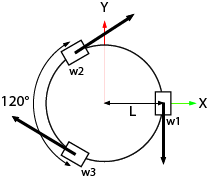
\includegraphics{figures/model}
	\caption*{FONTE: Própria}
\end{figure}

Robôs omnidirecionais tais como esse são particularmente úteis porque permitem
 maior manobrabilidade e eficiência, a um custo de maior complexidade na sua
 construção e controle. \cite{dynamical_models_for_omni_directional_robots}

\subsection{Modelagem Cinemática - Dedução da matriz por cinemática direta}

$\overrightarrow{V}$ é o vetor de velocidade linear do robô, $V_{w1}$, $V_{w2}$,
$V_{w3}$ são as velocidades lineares das rodas 1,2,3. 
$\omega $ é a velocidade angular do robô a partir do seu centro geométrico.
$L$ é a distância entre o centro de geométrico da roda e o centro de geométrico
do robô.

\begin{figure}[ht]
	\centering
	\caption{Diagrama do modelo matemático do robô, com valores dos ângulos das
	rodas}
	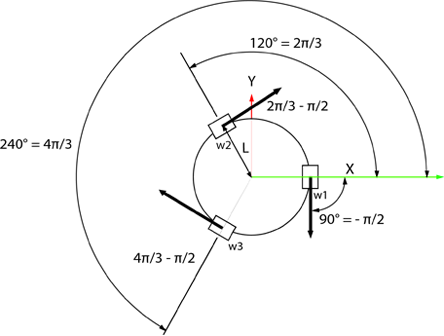
\includegraphics[width=0.8\textwidth]{figures/digram_model_dedution}
	\caption*{FONTE: Própria}
\end{figure}

\begin{equation}
    \begin{split}
        \overrightarrow{V}_{l} = 
        \overrightarrow{V}_{w1}
        + \overrightarrow{V}_{w2}
        + \overrightarrow{V}_{w3}
    \end{split}
\end{equation}

\begin{equation}
    \begin{split}
        \overrightarrow{\omega} = 
        \frac{\vert\overrightarrow{V}_{w1}\vert}{L}
        + \frac{\vert\overrightarrow{V}_{w2}\vert}{L}
        + \frac{\vert\overrightarrow{V}_{w3}\vert}{L}
    \end{split}
\end{equation}

\begin{gather*}
        V_{l} \angle \theta =  
        V_{w1} \angle \left(-\frac{\pi}{2}\right) 
        + V_{w2} \angle \left(\frac{2\pi}{3}-\frac{\pi}{2}\right) 
        + V_{w3} \angle \left(\frac{4\pi}{3}-\frac{\pi}{2}\right) 
\end{gather*}
\begin{gather*}
    V_{l} \cos{ \theta } + jV_{l} \sin{\theta} =  \\
    V_{w1} \cos{ \left(-\frac{\pi}{2}\right)} + jV_{w1} \sin{ \left(-\frac{\pi}{2}\right) } \\
    + V_{w2}  \cos{ \left(\frac{\pi}{6}\right) } + jV_{w2}  \sin{ \left(\frac{\pi}{6}\right) }  \\
    + V_{w3} \cos{ \left(\frac{5\pi}{6}\right) } + jV_{w3}  \sin{ \left(\frac{5\pi}{6}\right) } 
\end{gather*}

\begin{equation*}
    \begin{split}
        \omega = 
        \frac{V_{w1}}{L}
        + \frac{V_{w2}}{L}
        + \frac{V_{w3}}{L}
    \end{split}
\end{equation*}

\begin{gather}
	\begin{bmatrix} V\cdot \cos{\theta} \\  V\cdot \sin{\theta} \\  \omega \end{bmatrix}
	=
	\begin{bmatrix}
		\cos{\left(-\frac{\pi}{2}\right)} & \cos{\left(\frac{\pi}{6}\right)} & \cos{\left(\frac{5\pi}{6}\right)} \\
		\sin{\left(-\frac{\pi}{2}\right)} & \sin{\left(\frac{\pi}{6}\right)} & \sin{\left(\frac{5\pi}{6}\right)} \\
		\frac{1}{L} & \frac{1}{L} & \frac{1}{L}
	\end{bmatrix}
	\cdot
	\begin{bmatrix} V_{w1} \\  V_{w2} \\  V_{w3} \end{bmatrix}
\end{gather}

Matriz da cinemática direta:
\begin{gather}
	\begin{bmatrix}
		\cos{\left(-\frac{\pi}{2}\right)} & \cos{\left(\frac{\pi}{6}\right)} & \cos{\left(\frac{5\pi}{6}\right)} \\
		\sin{\left(-\frac{\pi}{2}\right)} & \sin{\left(\frac{\pi}{6}\right)} & \sin{\left(\frac{5\pi}{6}\right)} \\
		\frac{1}{L} & \frac{1}{L} & \frac{1}{L}
	\end{bmatrix}
	=
	\begin{bmatrix}
		0 & \sqrt{3}/2 & -\sqrt{3}/2 \\
		-1 & 1/2 & 1/2  \\
		1/L & 1/L & 1/L
	\end{bmatrix}
\end{gather}
Matriz inversa:
\begin{gather}
	\begin{bmatrix} V_{w1} \\  V_{w2} \\  V_{w3} \end{bmatrix}
	=
	\begin{bmatrix}
		0 & -2/3 & L/3 \\
		1/\sqrt{3} & 1/3 & L/3\\
		-1/\sqrt{3} & 1/3 & L/3
	\end{bmatrix}
	\cdot
	\begin{bmatrix} V\cdot \cos{\theta} \\  V\cdot \sin{\theta} \\  \omega \end{bmatrix}
\end{gather}
A matriz 3.5 é a matriz de cinemática do robô.
As entradas são o vetor velocidade linear e a velocidade angular do robô, e as
saídas são as velocidades lineares de cada uma das rodas.

Desconsiderando a velocidade angular, é possível observar os vetores velocidades
das rodas e o vetor velocidade linear do robô na figura \ref{simulacao}, que
foi gerada por meio de simulação em Python. O código fonte da simulação está
disponível em \url{https://github.com/dcarve/tg-robot/tree/master/simulation/vectors_simulation/src}.

\begin{figure}[ht]
	\centering
	\caption{Simulação dos vetores}
	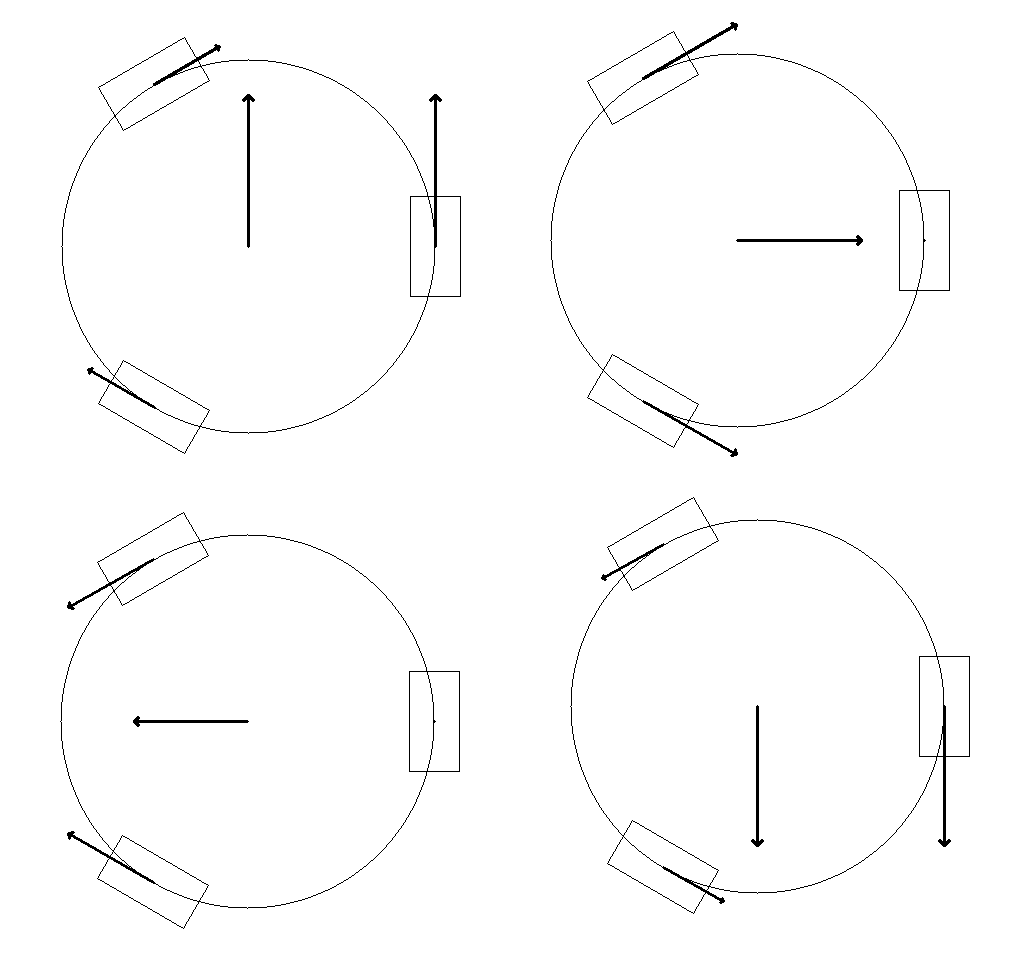
\includegraphics[width=0.7\textwidth]{figures/simulacao}
	\caption*{FONTE: Própria}
	\label{simulacao}
\end{figure}

\section{Roda Omnidirecional}

A roda omnidirecional aparece em vários modelos na literatura, tais como no design de J. Graboweicki em 1919
\cite{patent_US1305535A} e o de Josef Blumrich em 1972 \cite{patent_US3789947A}. A roda consiste de rolos
perpendiculares à  sua direção de giro, cuja presença tem como efeito conferir à roda a capacidade de se locomover em
qualquer direção no seu plano. Essa capacidade é o que confere aos robôs aqui discutidos suas características
holonômicas, uma vez que as restrições de movimento a que eles estão sujeitos está normalmente atrelada à construção dasrodas \cite{TAKAHASHI}.

\begin{figure}[h]
	\centering
	\caption{Modelo de uma Roda Omnidirecional}
	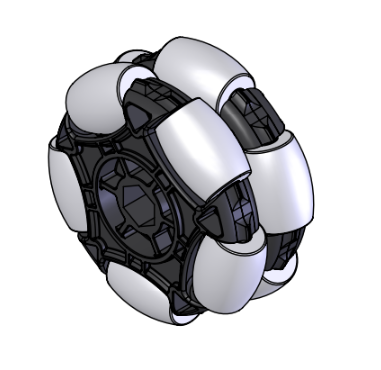
\includegraphics[width=0.5\textwidth]{figures/omniwheel}
    \caption*{FONTE: https://www.vexrobotics.com/omni-wheels.html}
\end{figure}

A relação entre velocidade linear e angular da roda é dada por:

\[V_{w1} = \omega_{w1}\cdot r \] 

em que $V_{w}$ é velocidade linear da roda, $r$ o raio da roda, $\omega_{w} $ e é a velocidade angular da roda.

Uma variação da roda omnidirecional é a roda mecanum, criada por Bengt Ilon \cite{patent_US3876255A} - 
a diferença fundamental entre elas é a construção dos rolos ligados à estrutura central  -
os quais, no caso da roda mecanum, são posicionados a 45°.

\subsection{Obtenção da roda omnidirecional}

Inicialmente foram compradas roda prontas, fabricas fora do território nacional, por meio de importação.
Mas o mesmo modelo pode ser encontrado sendo vendido no Brasil.
O modelo adquirido inicialmente possui diametro de 58mm, largura de 26mm e possui um acoplamento para eixo de 4mm de diametro.
Essas dimensões foram adquadas nos primeiros testes de contrução do robô enquanto se estava usando motores DC,
mas quando o projeto passou a usar motores de passo Nema 17, as rodas não eram mais compatíveis com o eixo e as dimensões dos motores.
(A mudança de tipos de motores será discutida na seção sobre motores).

\begin{figure}[h]
	\centering
	\caption{Roda omnidirecional usada inicialmente}
	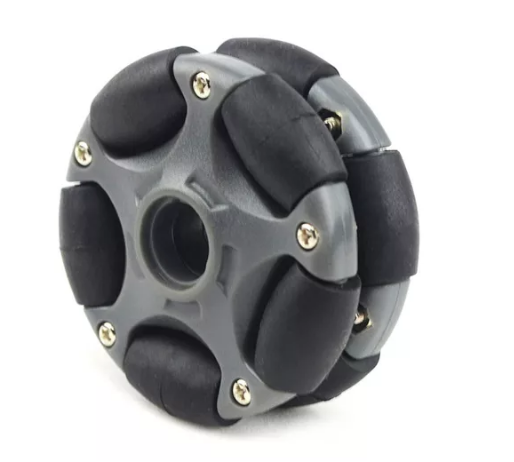
\includegraphics[width=0.5\textwidth]{figures/roda_china.png}
    \caption*{FONTE: https://rapidroboticsaustralia.com/products/58mm-nylon-omni-directional-wheel-4mm-hub}
\end{figure}

A mudança de requisitores para as rodas levou a criar um design próprio e fabricado com impressoa 3d,
parafusos sextavado de M3, e reutilizando os rolamentos das rodas de 58mm.
As novas rodas possuem 69mm de diametro e 27mm de largura, fabricadas com filamento PLA.

\begin{figure}[h]
	\centering
	\caption{Processo de desing da nova roda - AutoCAD}
	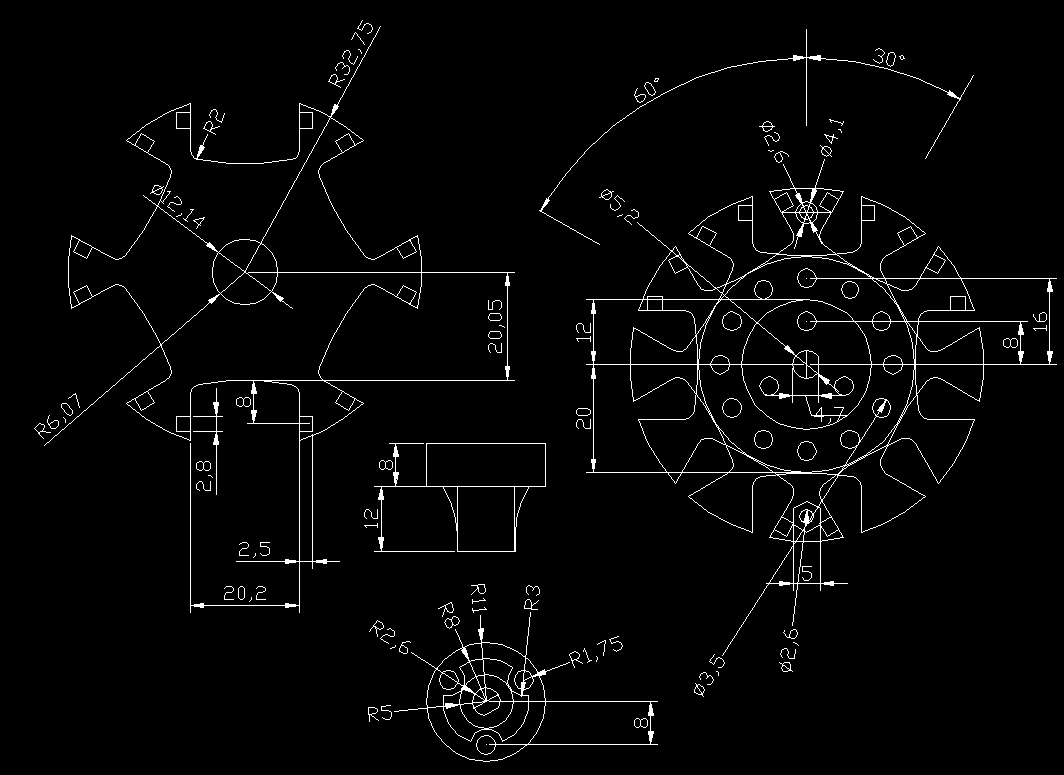
\includegraphics[width=0.9\textwidth]{figures/roda_processo_desing_passo1}
    \caption*{FONTE: Própria}
\end{figure}

\begin{figure}[h]
	\centering
	\caption{Estudo e testes do design da nova roda}
	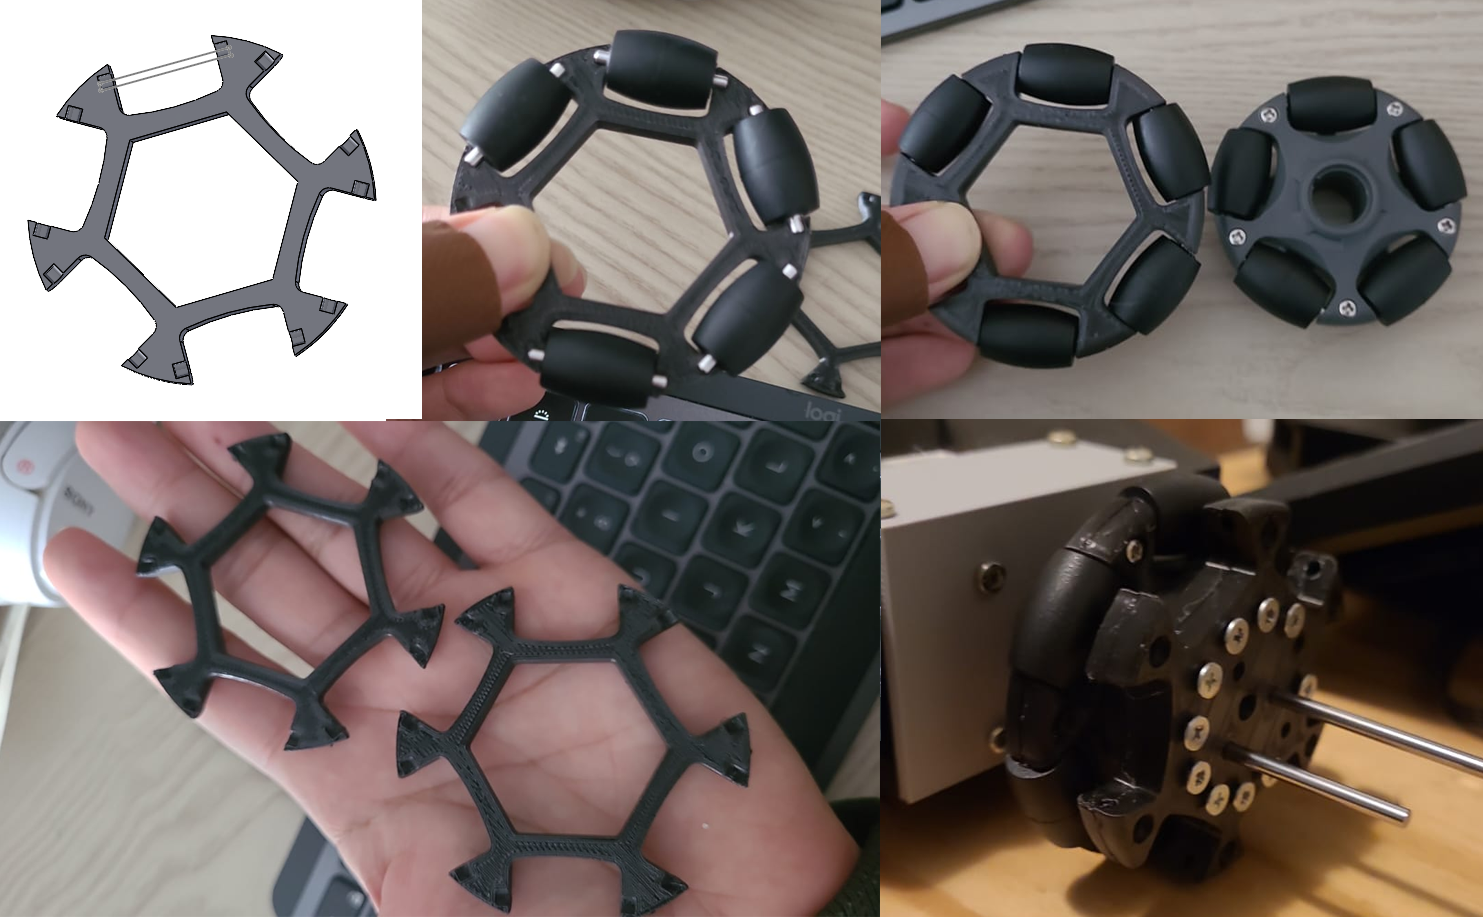
\includegraphics[width=0.9\textwidth]{figures/estudo_roda}
    \caption*{FONTE: Própria}
\end{figure}

\begin{figure}[h]
	\centering
	\caption{Desing final - Solidworks}
	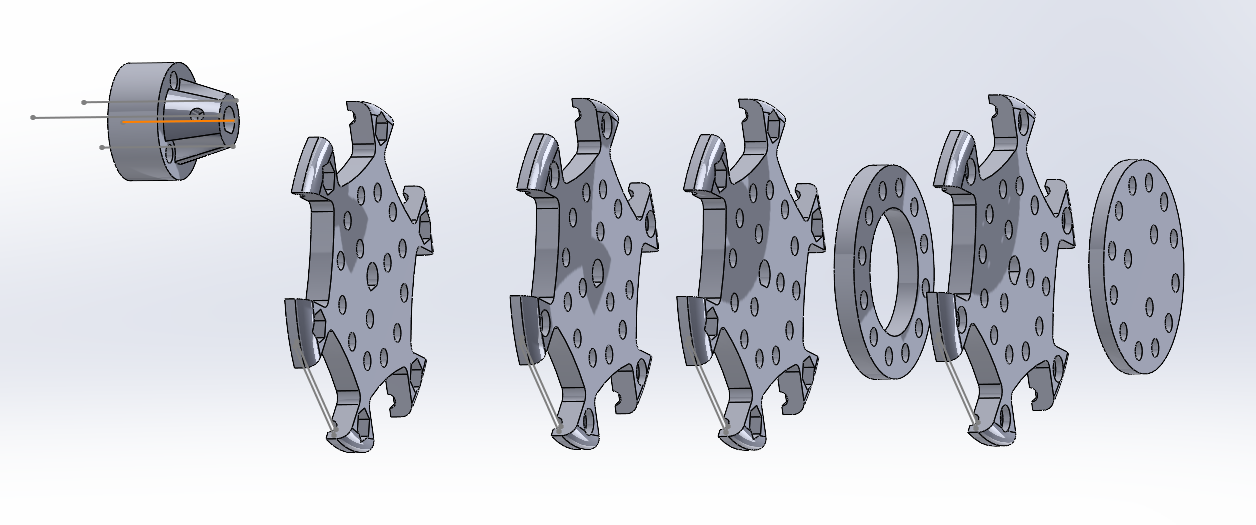
\includegraphics[width=0.9\textwidth]{figures/roda_processo_desing_passo2}
    \caption*{FONTE: Própria}
\end{figure}

\begin{figure}[h]
	\centering
	\caption{Desing final - Preparação para impressão}
	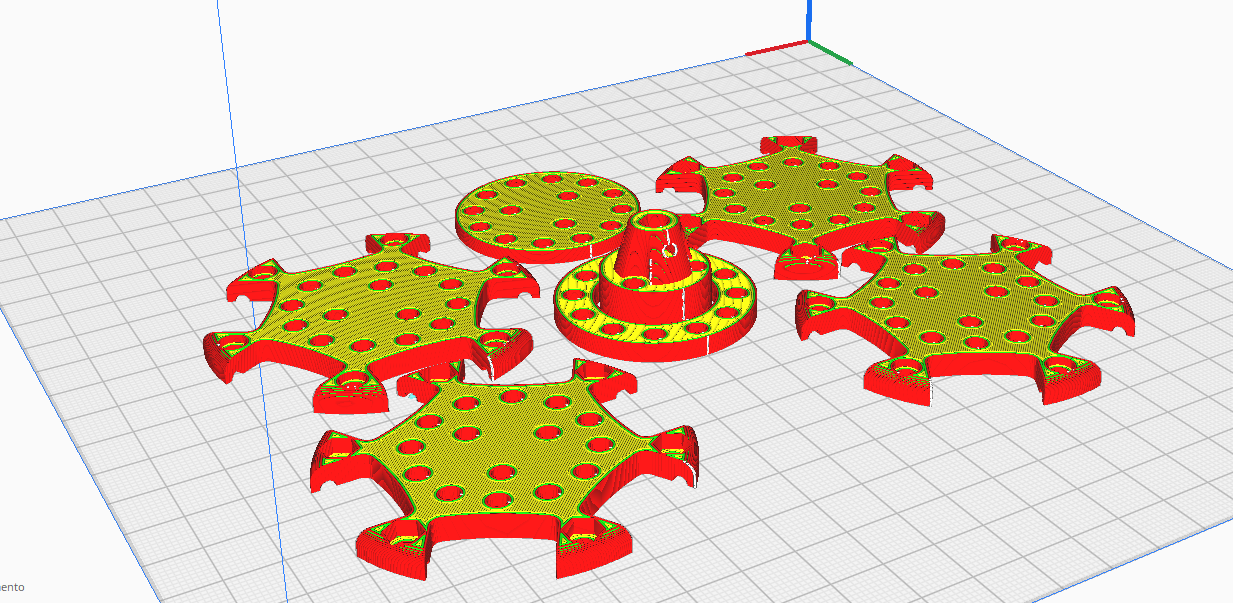
\includegraphics[width=0.9\textwidth]{figures/roda_processo_desing_passo3}
    \caption*{FONTE: Própria}
\end{figure}

\begin{figure}[h]
	\centering
	\caption{Montagem da roda}
	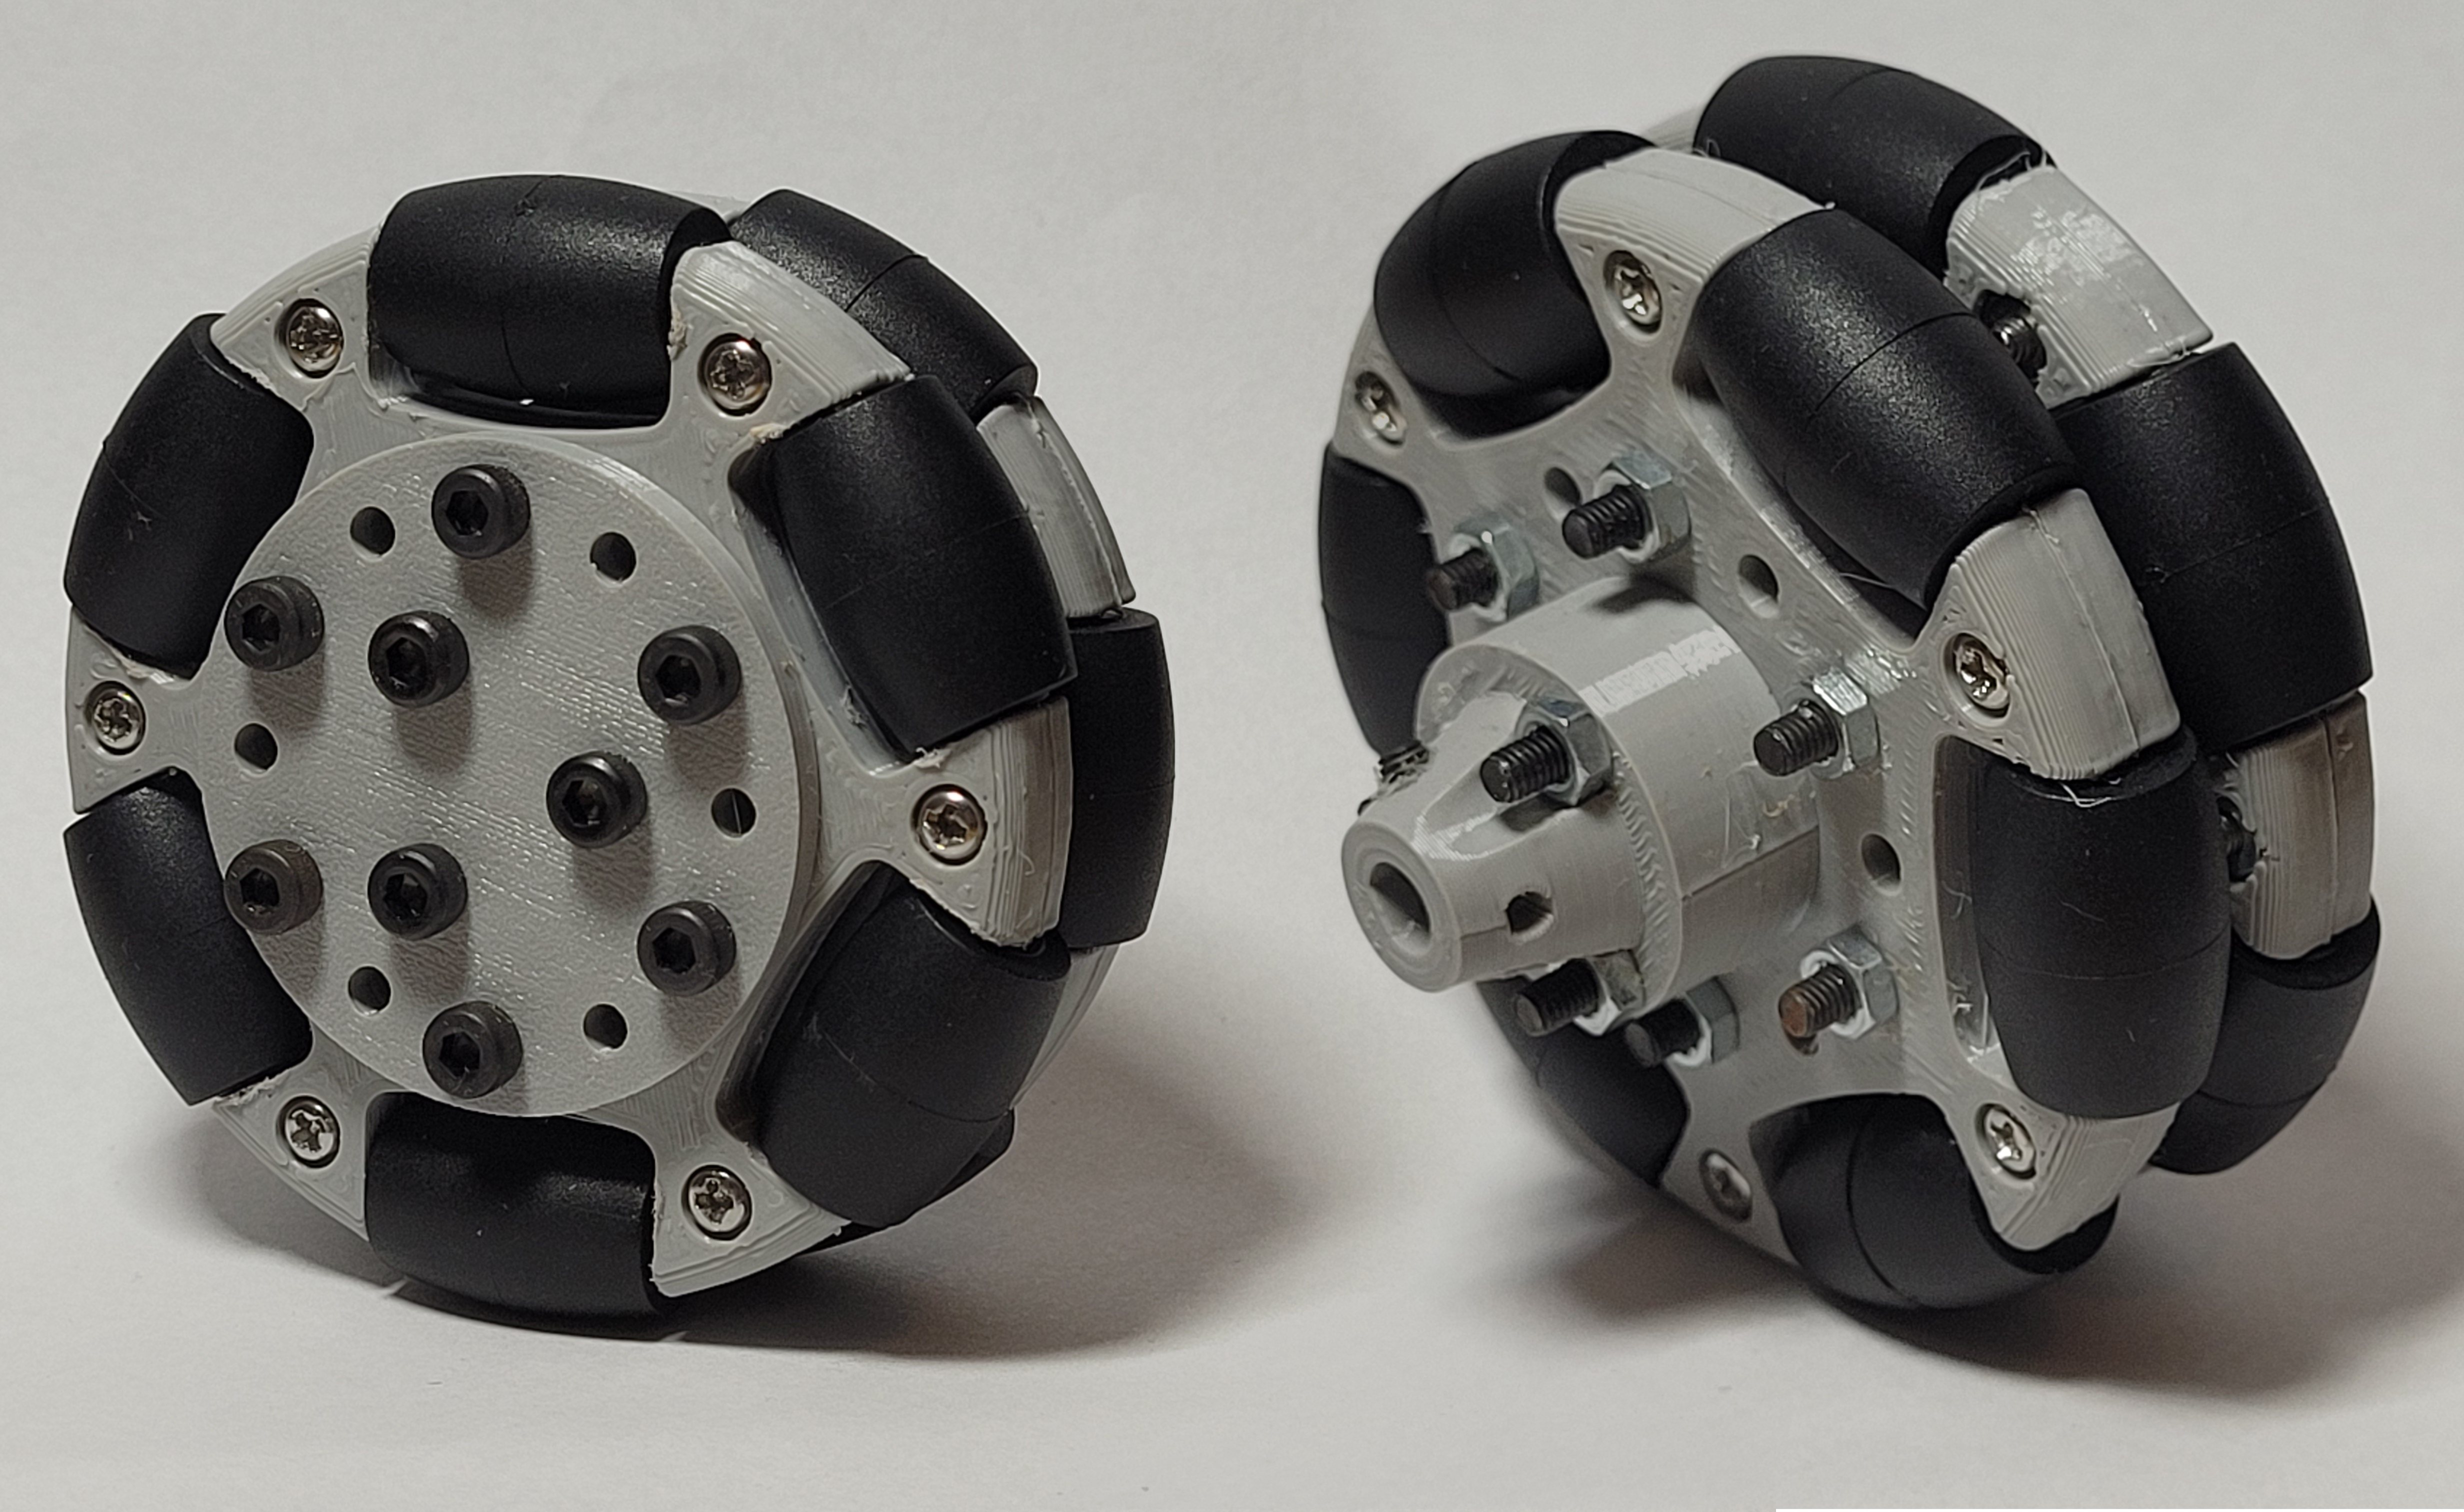
\includegraphics[width=0.9\textwidth]{figures/roda_processo_desing_passo4}
    \caption*{FONTE: Própria}
\end{figure}

\section{Microcontrolador e IDE}

\subsection{Microcontrolador}

Microcontroladores são circuitos integrados compactos desenvolvidos para governar
uma operação específica em um sistema embarcado. No contexto da aplicação deste
trabalho, o uso de um microcontrolador é fundamental para se obter o controle
desejado de trajetória e posicionamento do robô.

Foram testadas duas placas de microcontrolador o BluePill e ESP32 Devkit v1
Ambas com processadores de 32bits
e podem ser alimentadas através dos pinos de 5v e 3.3v, mas também através do connector micro-USB-B

A escolha dessas duas placas durante o desenvolvimento foi motivada pelo custo de aquisição
e pelos componentes e opções de comunicação disponíveis.
Já se era conhecido o baixo preço da placa BluePill, e já havia sido adquirido anteriormente ao projeto.
A escolha do ESP32 Devkit v1 foi motivada também pelo custo, mas também pela
integração com bluetooth que será discutida nas seções a seguir.

A tabela \ref{precos_placas} compara a faixa de preço entre as principais placas de desenvolvimento
que podem ser encontradas para compra em território nacional.

\begin{quadro}[htb]
	\caption{Comparação de preços entre as placas de desenvolvimento \label{precos_placas}}
	 \begin{tabular}{|c|c|}
		\hline
		\textbf{Placa de desenvolvimento} & \textbf{Faixa de preço em R\$} \\ \hline
		BluePill (STM32F103C8T6) &  23 - 49 (já adquirido anteriormente) \\ \hline
		ESP32 DevKit V1  &  40 - 80   \\ \hline
		Arduino Due R3 &  320 - 470   \\ \hline
		Nodemcu v3 ESP8266 & 22 - 35   \\ \hline
		Raspberry pi pico (1, 2, W, H)  & 36 - 66  \\ \hline
	\end{tabular}
	\caption*{FONTE: Própria}
\end{quadro}

A pesquisa de preços foi feita nas principais lojas de componentes eletrônicos disponível online:
\begin{itemize}
	\item https://www.rsrobotica.com.br/
	\item https://www.robocore.net/
	\item https://www.makerhero.com/
	\item https://www.iot-robotica.com.br/
	\item https://www.ardurobotica.com.br/
	\item https://curtocircuito.com.br/
	\item https://www.saravati.com.br/
	\item https://www.a2robotics.com.br/
	\item https://www.ardurobotica.com.br/
	\item https://www.casadarobotica.com/
\end{itemize}



\subsubsection{BluePill - STM32F103C8}

A placa BluePill embarca o microcontrolador STM32F103C8.
"STM32" é uma família de microcontroladores de 32-bits fabricados pela
ST-Microelectronics. O processador empregado nessa família é o ARM Cortex-M3 \cite{cortex_m3},
baseado em arquitetura Harvard. Tem 64Kbs de memória flash.

De acordo com o \textit{livro Discovering the STM32 Microcontroller} \cite{stm_doc} e 
a documentação colaborativa do projeto STM32-base.org \cite{stm32_base_org},
possui também 7 timers, 2 ADCs, e 9 interfaces de comunicação, incluindo I2C,  USART, SPI, e USB 2.0. 
O STM32 apresenta 7 pinos que suportam canais de PWM de 5V, e outros 8 canais de 3.3V, e pode ser alimentado
via microUSB de 5V. Existem 3 grupos de pinos,  $P_{A}$,  $P_{B}$ e  $P_{C}$: os pinos PA vão de $P_{A0}$ 
a $P_{A15}$, PB indo de $P_{B0}$ a $P_{B15}$, e PC com apenas 3 pinos, $P_{C13}$, $P_{C14}$ e $P_{C15}$.
A relação geral dos pinos pode ser melhor obervada na figura \ref{stm32f103c8_pinout}.

\begin{figure}[ht]
	\centering
	\caption{Diagrama de pinos do STM32F103C8}
	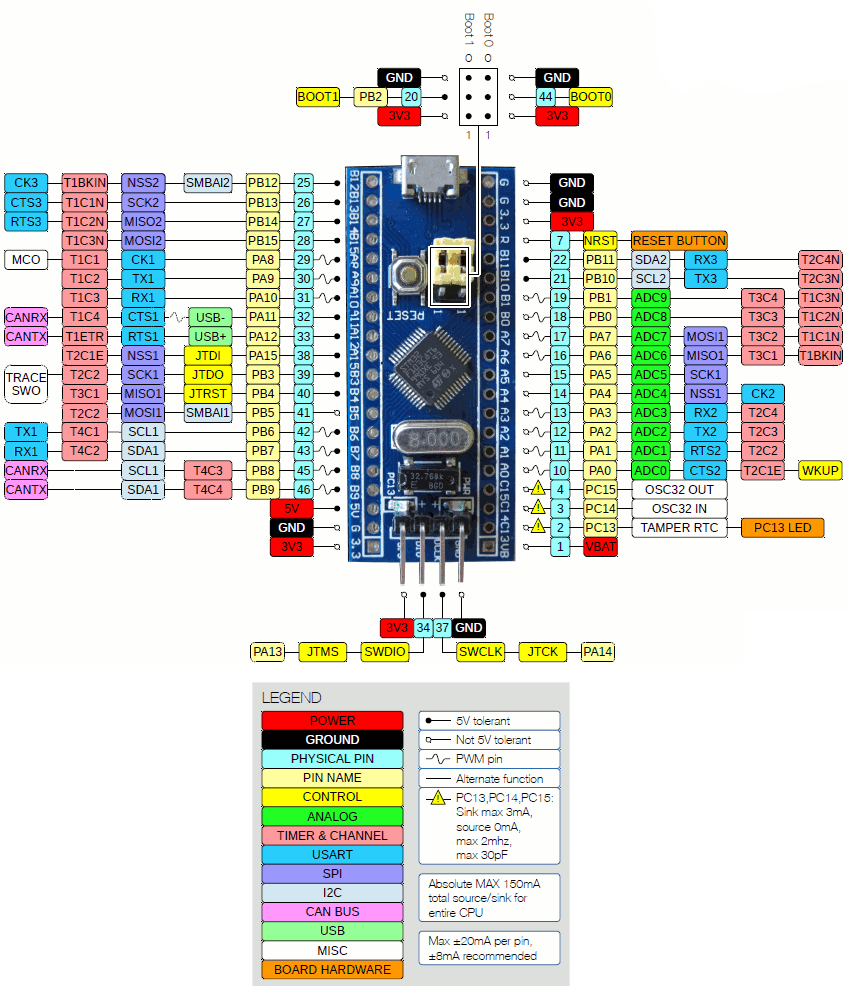
\includegraphics[width=1.0\textwidth]{figures/stm32f1_pinout}
	\caption*{FONTE: Sistemas Microprocessados -Apostila com práticas e foco nos processadores ARM CORTEX \cite{apostila_microprossados}}
    \label{stm32f103c8_pinout}
\end{figure}

Para carregar o projeto no microcontrolador, tem por padrão o uso do gravador ST-LINK v2.
O ST-link, cujo original (figura \ref{stlinkv2_original}) é fabricado pela ST-Microelectronics, 
possui uma versão paralela mais barata
comercializada online (figura \ref{stlinkv2_cheap}), porém a versão paralelo costuma ter fabricantes diversos e 
muitas vezes não descritos na distribuição do produto 
e a relação de pinos pode variar (figura \ref{stlinkv2_cheap_pin_diff}).

É possível modificar o firmware do STM32F103C8 para permitir grava-lo via USB, porém esse procedimento
não é algo disponibilizado pela ST-Microelectronics, sendo necessário utilizar ferramentas de terceiros,
muitas vezes de projeto de código aberto que não possuem mais suporte \cite{stm32duino_bootloader}.
A conexão micro-USB-B ainda funciona como uma comunicação serial e poder ser usada como uma porta serial que pode ser usada para debug
mas se usada ao mesmo tempo que o ST-link pode danificar o microcontrolador, já que o regulador estará rebendo 5v da entrada USB
e disponilizando 3.3v volts, mas 3.3v também estão sendo disponibizados direto do ST-link.

\begin{figure}[ht]
	\centering
	\caption{St-Link V2 original fabricado pela ST-Microelectronics \cite{st_link_v2}}
	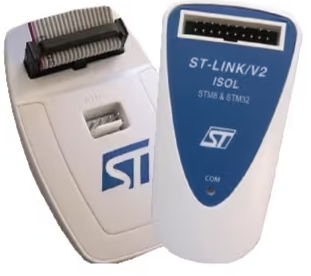
\includegraphics[width=0.5\textwidth]{figures/stlinkv2_original}
	\caption*{FONTE: ST-Microelectronics - ST-Link V2}
    \label{stlinkv2_original}
\end{figure}


\begin{figure}[ht]
	\centering
	\caption{St-Link V2 paralelo de fabricação desconhecida \cite{stlinkv2_cheap_ref}}
	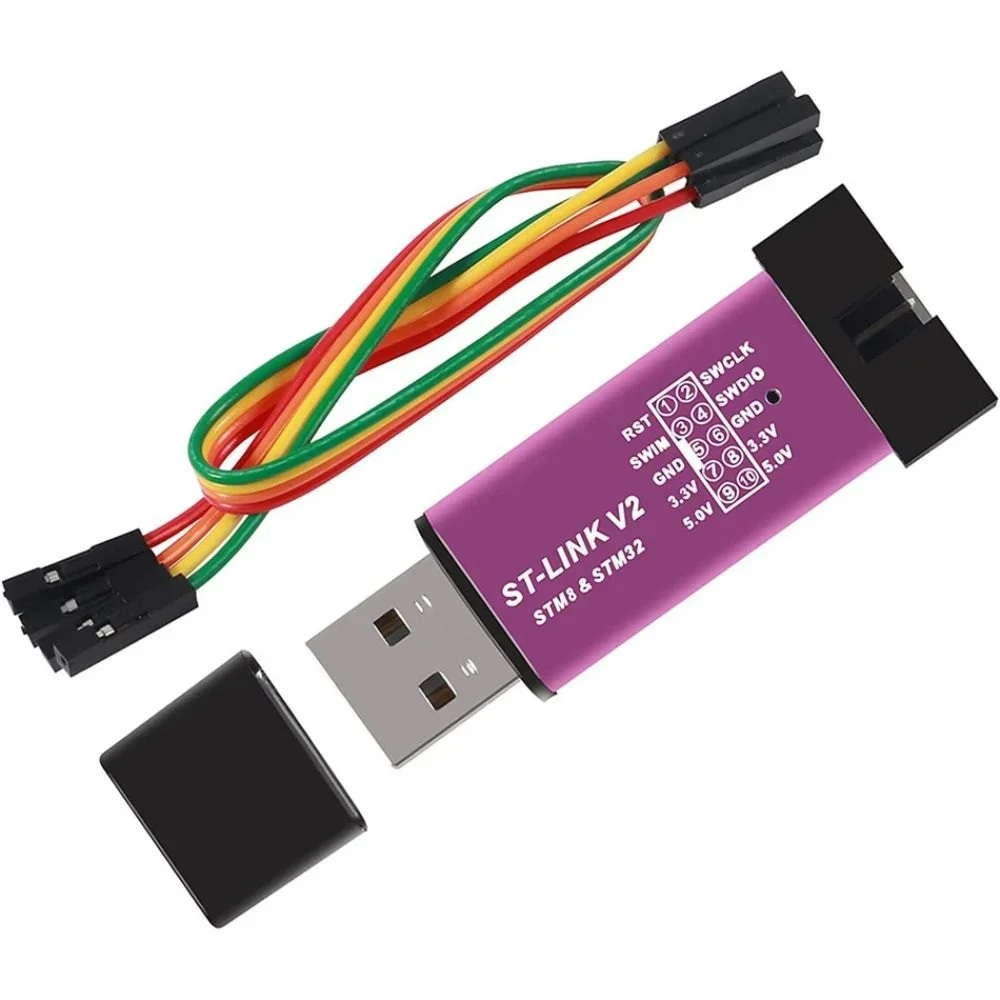
\includegraphics[width=0.5\textwidth]{figures/stlinkv2_cheap}
	\caption*{FONTE: https://www.achavevirou.com.br/gravador-st-link-v2-para-stm32-e-stm8}
    \label{stlinkv2_cheap}
\end{figure}


\begin{figure}[htb]
	\centering
	\caption{St-Link V2 paralelo e o problema da não padronização de pinos}
	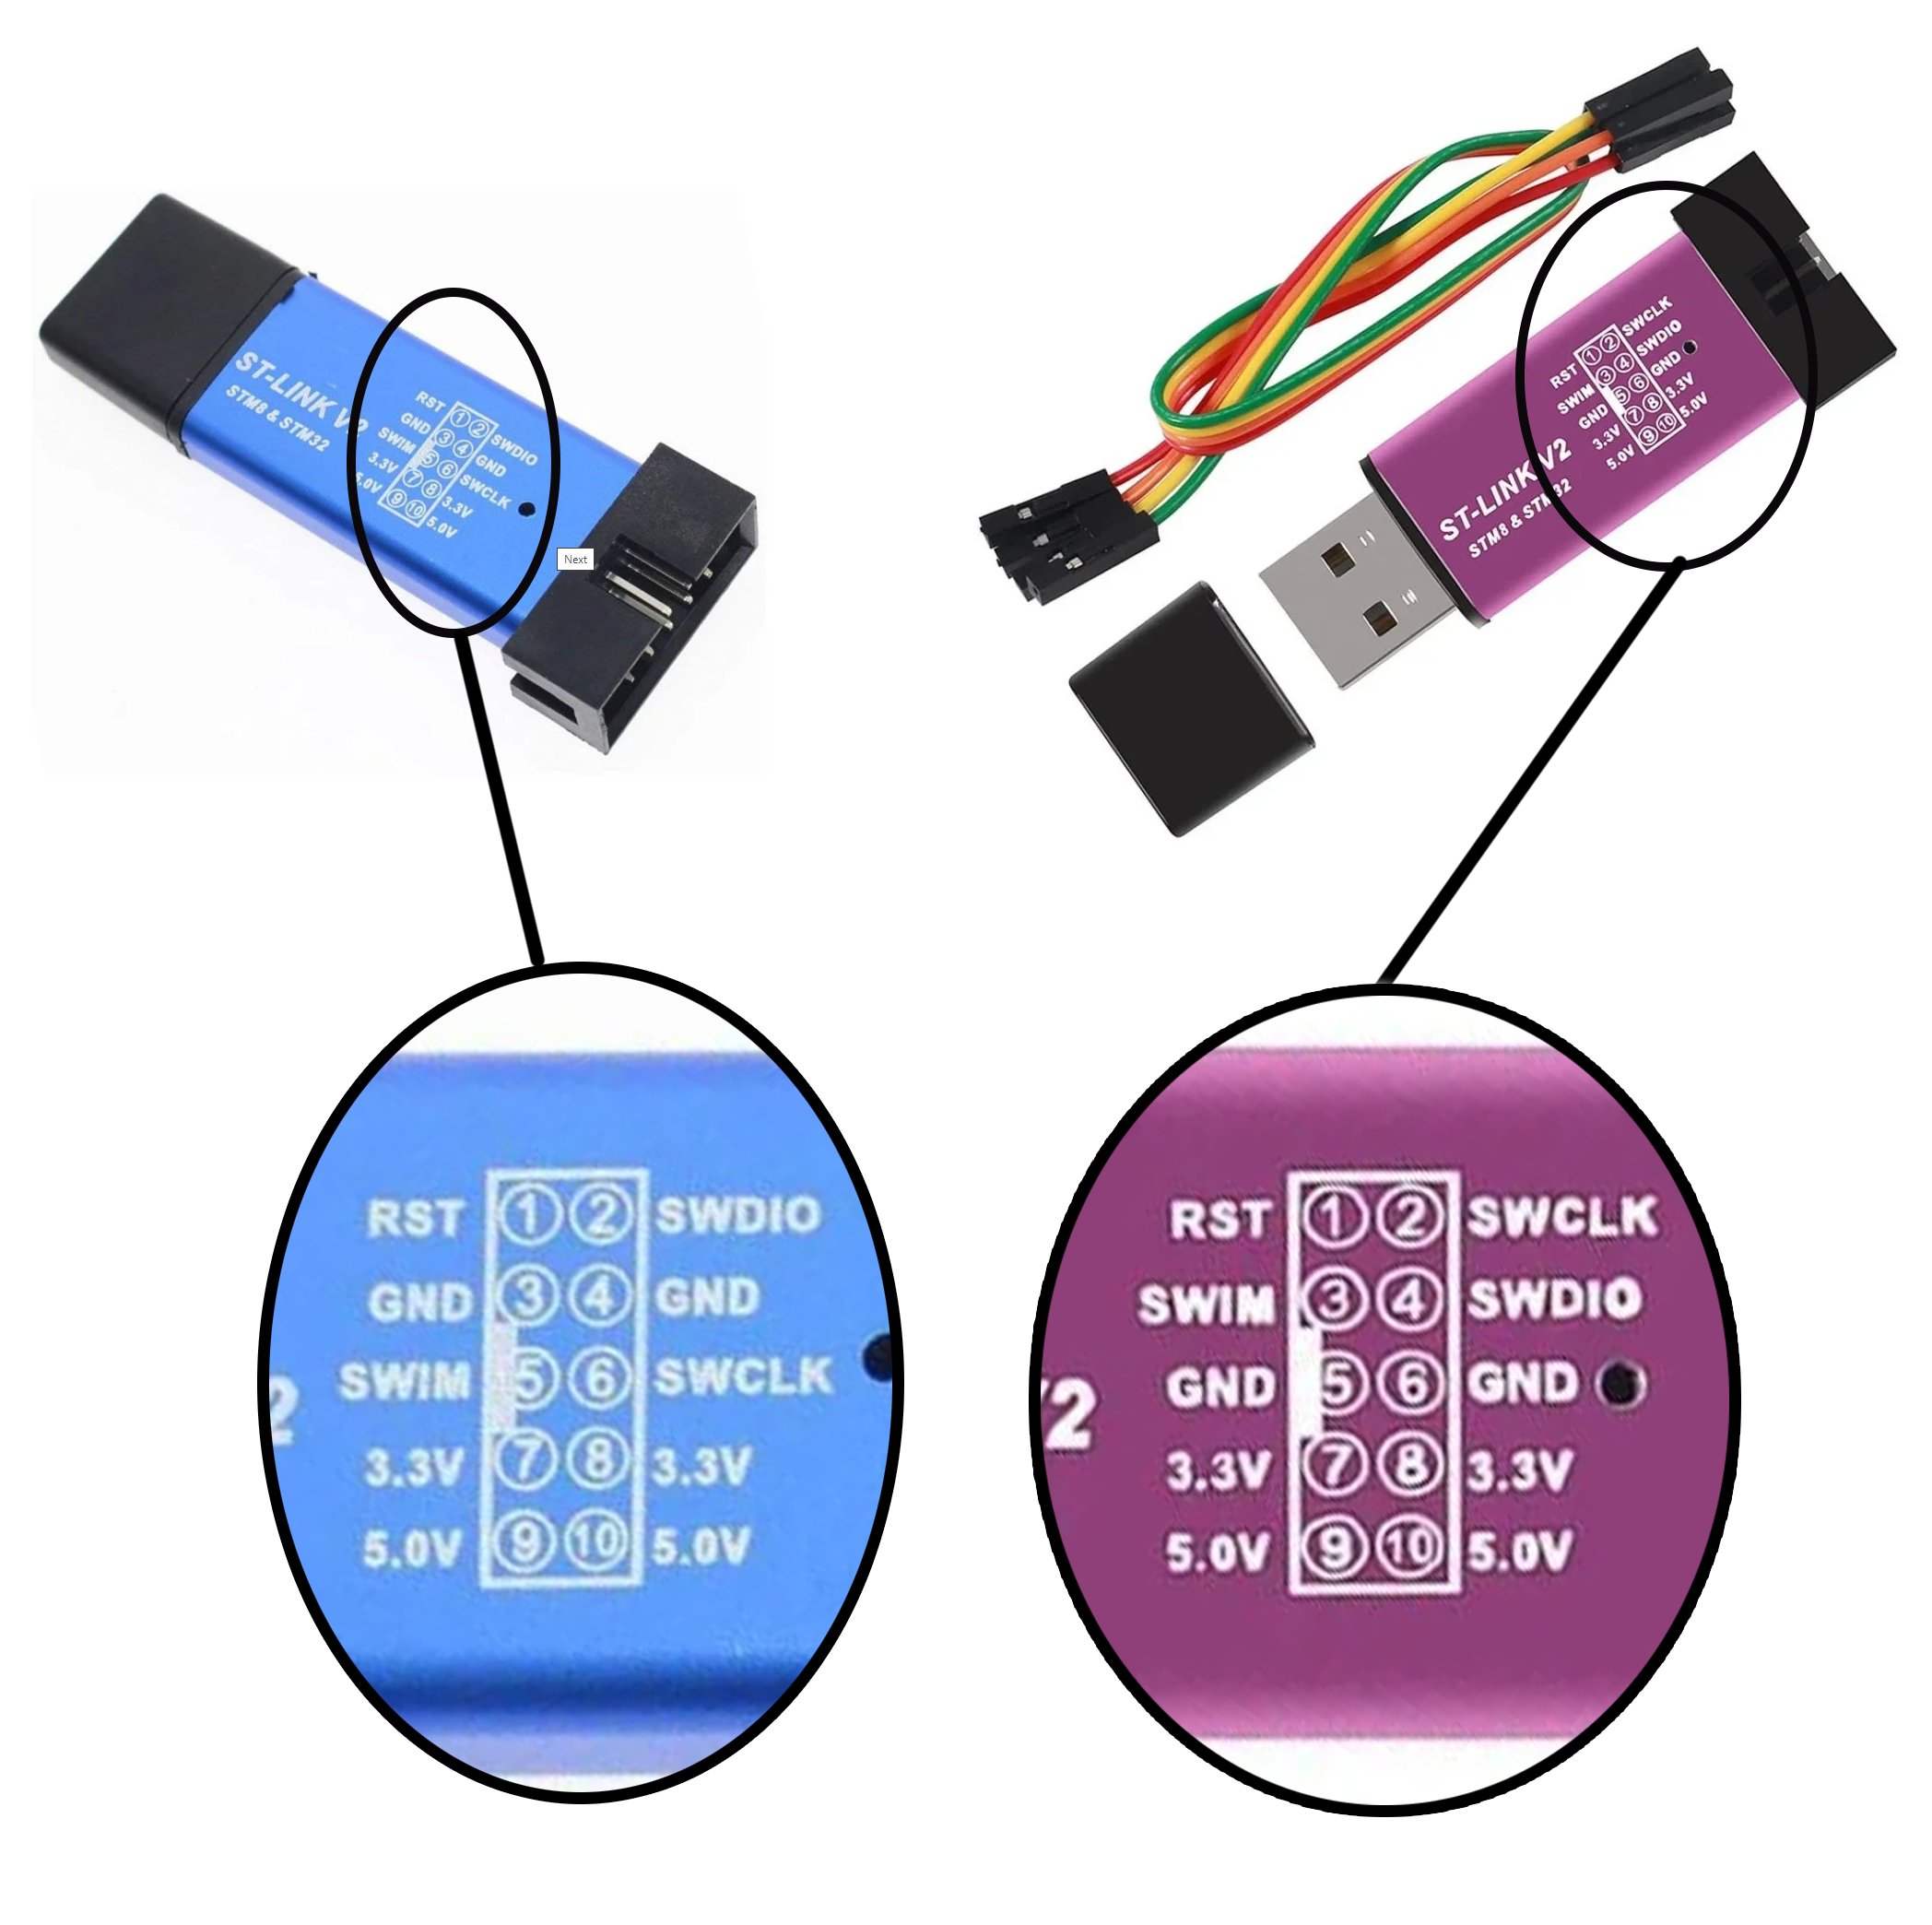
\includegraphics[width=0.5\textwidth]{figures/stlinkv2_cheap_pin_diff}
	\caption*{
		FONTE: Adaptado de https://universal-solder.ca/st-link-v2-usb-programmer-debugger/
		e https://www.achavevirou.com.br/gravador-st-link-v2-para-stm32-e-stm8
	}
    \label{stlinkv2_cheap_pin_diff}
\end{figure}

A partir desse ponto todas as menções a "STM32" são referem diretamente a  placa BluePill.


\subsubsection{ESP32 Devkit v1}

A placa ESP32 Devkit v1, de fabricação da DOIT.am, ela possui o microcontrolador ESP32-WROOM-32E (figura \ref{esp32_pinout}) fabricado pela Espressif Systems
A série ESP32 foi lançada em 2016 \cite{anuncio_esp32}, e possui arquitetura de 32 bits
tem se tornado popular por possuir opções com integração bluetooth e wifi.
O ESP32-WROOM-32E possui um processador dual core ESP32-D0WD-V3 \cite{esp32_wroom_32e_datasheet}, com frequência máxima de 240MHz, wi-fi 2.4Ghz de até 150Mbps e
bluetooth 4.2. Em relação aos periféricos, embora a placa tenha 48 GPIOs, elas estão endereçadas em apenas 25 pinos.
Entre os periféricos existem 15 canais ADC, 2 interfaces UART, 
2 canais DAC, 25 PWM, uma interfade de SPI, I2C e I2S, e 9 interface de toque capacitivo \cite{esp32_reference_2} \cite{esp32_reference}.

\begin{figure}[ht]
	\centering
	\caption{Diagrama de pinos do ESP32 Devkit v1}
	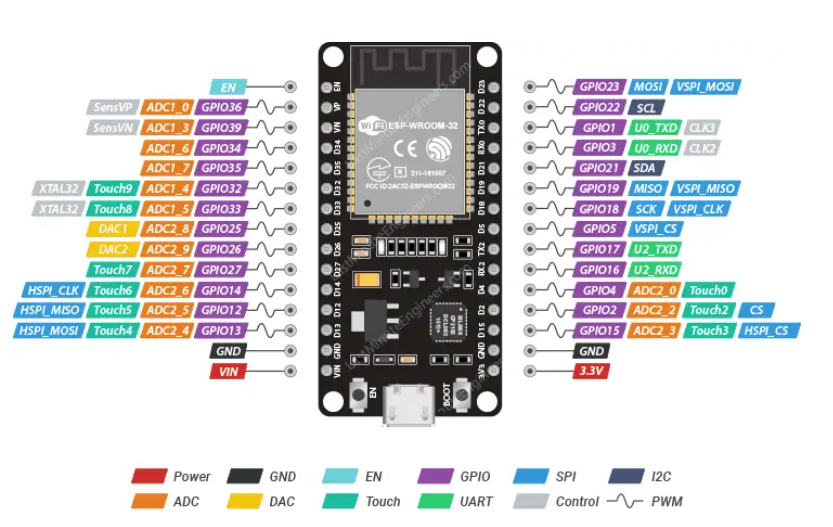
\includegraphics[width=1.0\textwidth]{figures/esp32_pinout}
	\caption*{FONTE: Adaptado https://lastminuteengineers.com/esp32-pinout-reference/}
	\label{esp32_pinout}
\end{figure}

De acordo com alguns artigos dispoíveis online sobre o ESP32 Devkit v1  \cite{esp32_reference_2} \cite{esp32_reference},
nem todos os 25 pinos são totalmente livres para usar,
alguns possuem limitações de uso de acordo como periférico em uso, a figura \ref{esp32_pinout_ref} resume as recomendações de uso do pinos.
Diferente do STM32 o ESP32 Devkit v1 pode ser gravado diretamente via USB.

\begin{figure}[ht]
	\centering
	\caption{Recomendação de uso dos pinos do ESP32 Devkit v1}
	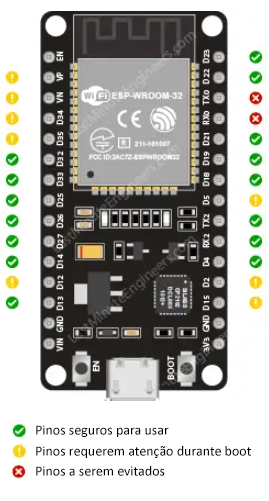
\includegraphics[width=0.35\textwidth]{figures/esp32_pinout_ref}
	\caption*{FONTE: Adaptado https://lastminuteengineers.com/esp32-pinout-reference/}
	\label{esp32_pinout_ref}
\end{figure}

A partir desse ponto todas as menções a "ESP32" são referem diretamente a placa ESP32 Devkit v1.


\subsection{IDE}

\subsubsection{Atollic TrueSTUDIO}

\begin{figure}[ht]
	\centering
	\caption{Interface Atollic}
	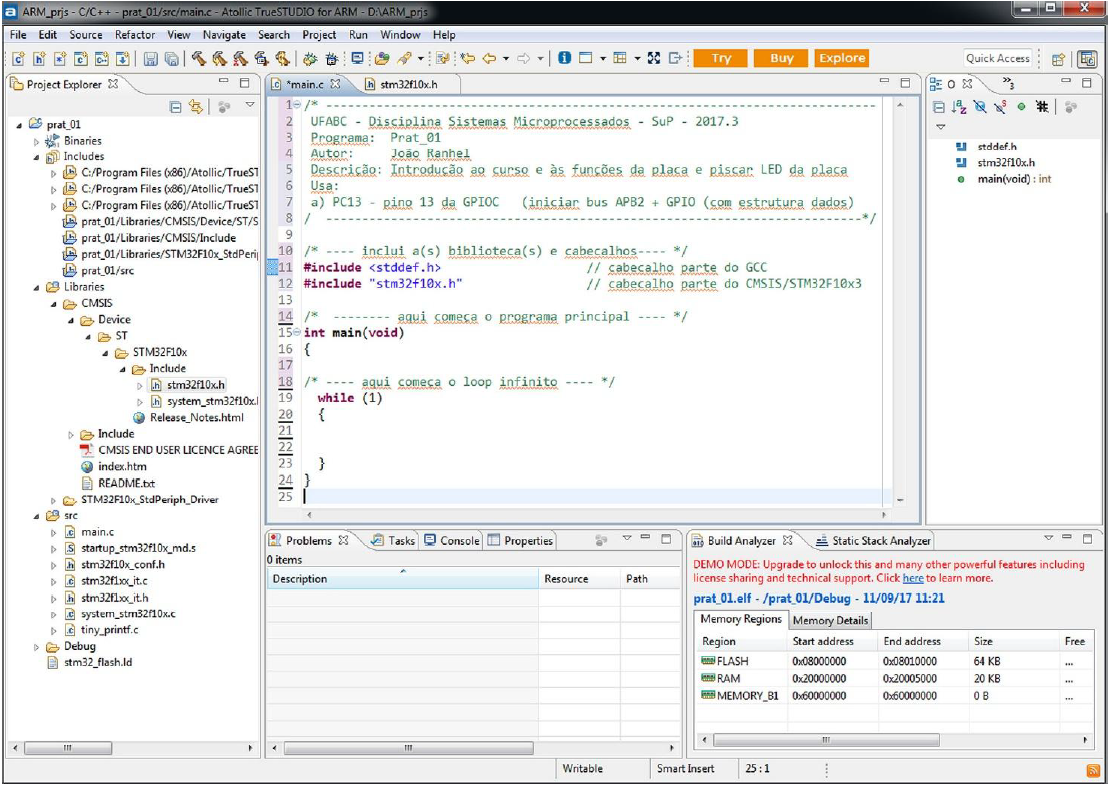
\includegraphics[width=0.8\textwidth]{figures/atollic}
	\caption*{FONTE: Sistemas Microprocessados -Apostila com práticas e foco nos processadores ARM CORTEX \cite{apostila_microprossados}}
\end{figure}

A IDE a ser usada para programar um STM32 seria o TrueSTUDIO, distribuído pela
Atollic, que foi adquirida pela ST-Microelectronics em 2017. Trata-se de um
software livre para programar em C/C++, criado com base na plataforma Eclipse,
e que possui todas as funções esperadas para o trabalho com o STM32, tais como
edição, compilação e debugging. Uma de seus principais vantagens é não haver
limites para tamanho de projeto, o que o torna ideal para trabalhos
profissionais. O TrueSTUDIO deixou de receber atualizações em 2017,
depois da aquisição pela ST-Microelectronics.\cite{apostila_microprossados}


\subsubsection{Arduino IDE}

Criado para ser a IDE das placa de desevolvimento Arduino, a primeira versão foi criada em 2005 \cite{arduino_id_history},
Mas as versões mais populares dispobilizadas ao público, são a 1.0.6 e 1.8. 
A versão 1.8 foi lançada em 2016 e recebeu atualizações até 2021, 
com a versão 2.0.0 lançada em 2022 \cite{arduino_tag_2}.

\begin{figure}[ht]
	\centering
	\caption{Interface Arduino}
	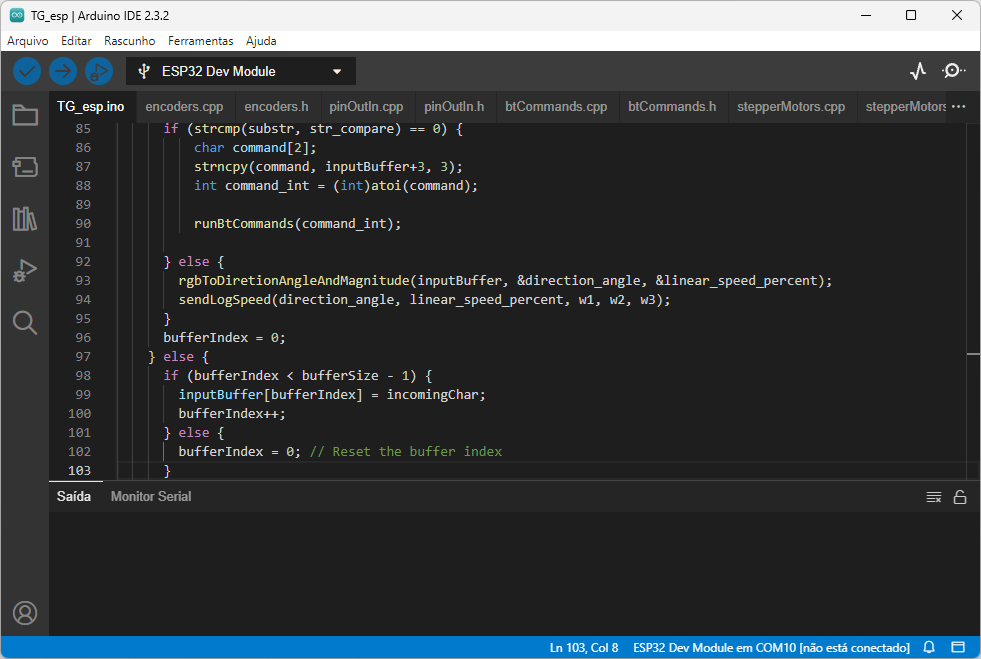
\includegraphics[width=0.9\textwidth]{figures/arduino}
	\caption*{FONTE: Própria}
\end{figure}

\subsection{Escolha do microcontrolador e IDE}

\subsubsection{IDE}

Devido a complicações nas configurações de múltiplas saídas de PWM com o
TrueSTUDIO, optou-se por usar Arduino como alternativa. Um obstáculo a essa
alternativa é que o Arduino não é compatível com STM32 nativamente,
porém o projeto Arduino\_STM32 \cite{arduino_stm32}, por Roger Clark.
O projeto contem os arquivos em C para usar o hardware do STM32 com Arduino IDE
do STM32 no Arduino. No momento de escrita deste trabalho, o projeto era
compatível apenas com a versão 1.8 da IDE do Arduino.

A escolha de usar a IDE do Arduino logo se tornou uma opção mais viável e flexível.
seja pela vasta lista  bibliotecas disponibilizadas por contribuidores e
documentações de projetos independentes. 

A IDE também é compatível com o ESP32,  usando a biblioteca arduino-esp32 \cite{arduino_esp32},
disponibilizada e mantida atualizada pela Espressif Systems.

\subsubsection{Microcontrolador}

Durante o desenvolvimento, o projeto foi migrado do STM32 para o ESP32 
devido a limitação do STM32 não poder ser conectado a porta serial via micro-USB-B e ST-link ao mesmo tempo,
e também de não poder deixar ligado o módulo HC-05 durante a gravação no STM32.
Sobre o módulo HC-05, em específico aos pinos de comunicação serial, se os pinos tiverem algum comportamento
diferente do padrão durante a gravação de um novo programa, esse comportamento pode danificar o módulo,
durante os teste, dois módulos foram danificados devido a excessivas vezes em que foram deixados
conectados ao STM32 durante a gravação de um novo programa.
E durante o uso STM32, algumas vezes a conexão via micro-USB-B permaneceu ligada ao mesmo tempo que o ST-link. 
A ocorrência excessiva dessa conexão levou a danificação do STM32.

Considerando esses pontos das diculdades encontradas com o uso do STM32, conexão via micro-USB-B e o módulo HC-05,
a placa ESP32 se tornou uma opção mais prática, pois já vinha integrado com bluetooth e podiaria ser conectado via micro-USB-B
para gravação e comunicação serial para debug ao mesmo tempo. E não seria necessário mudar de IDE e
seria necessário pouca alteração no projeto para adaptar o uso do bluetooth nativo.

\section{Comunicação com o robô}

Como o plano original era usar o microcontrolador STM32,
a comunicação mais simples e direta de implementar seria uma comunicação serial com um módulo Bluetooth.
Foi considerando comunicação via rádio, porém exigiria um investimento na aquisição de um controle RC.
Uma comunicação Bluetooth exige apenas a integração de um aplicação Android para enviar dados via Bluetooth.

\subsection{Módulo HC-05 vs ESP-WROOM-32}

Na seção \ref{microcontrolador_ide} foi discutido a mudança do microcontrolador STM32 para o ESP32.
e como o uso do módulo HC-05 exigia um nível de atenção maior ao escrever um novo programa no STM32.
A alteração para o ESP32, com o chip ESP-WROOM-32 (com Bluetooth e Wi.fi integrado) não exigiu muitas alterações no projeto.
Pois, o componente Bluetooth é controlado como se fosse uma comunicação serial.

\noindent
\begin{minipage}[t]{0.48\textwidth}
\captionsetup{labelformat=empty}
\begin{lstlisting}[
    language=C,
    caption={Comunicação entre STM32 e HC-05}
]
#include <HardwareSerial.h>
#include <libmaple/usart.h>

void setup() {
    pinMode(RX_STM_PIN, INPUT);
    pinMode(TX_STM_PIN, OUTPUT);
    Serial3.begin(9600);
    Serial.begin(9600);
};
\end{lstlisting}
\end{minipage}
\hfill
\begin{minipage}[t]{0.48\textwidth}
\captionsetup{labelformat=empty}
\begin{lstlisting}[
    language=C,
    caption={Comunicação com Bluetooth integrado}
]
#include "BluetoothSerial.h"

BluetoothSerial SerialBT;

void setup() {
    SerialBT.begin("deviceName");
    Serial.begin(115200);
};
\end{lstlisting}
\end{minipage}

\subsection{Aplicativo Android}

\subsubsection{Controle de direção}

O aplicativo Arduino Bluetooth Controller possui uma opção em que o aplicativo envia uma
'string' representando as cores RGB em 'int8'.
por exemplo,  vermelho seria '255000000' (r=255, g=0, b=0).
E a interface é o modelo de cor HSV em 2 dimensões de ponta cabeça,
\autoref{arduino_bluetooth_controller_hsl_model}.


\begin{figure}[ht]
	\centering
	\caption{Tela de controle RGB do aplicativo Arduino Bluetooth Controller}
	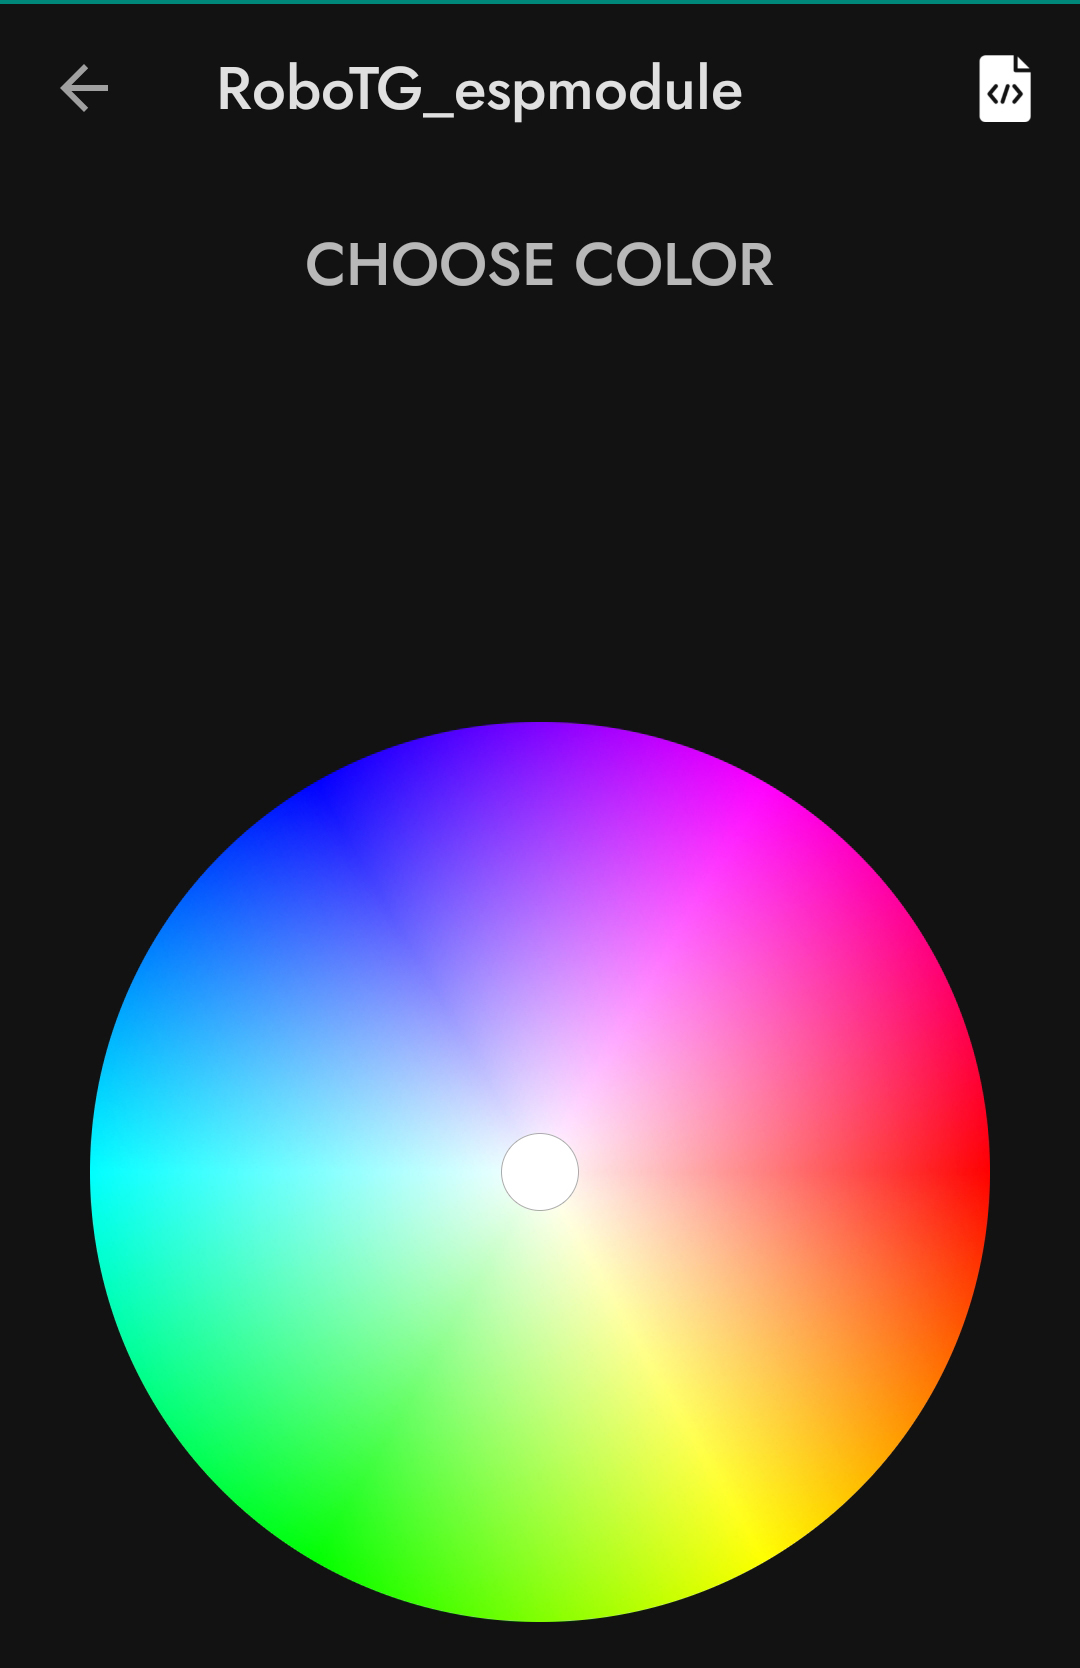
\includegraphics[width=0.40\textwidth]{figures/andriod_bluetooth_controller_hsl_model}
	\fonte{Própria}
	\label{arduino_bluetooth_controller_hsl_model}
\end{figure}

No modelo HSV,  a \autoref{rbg_hsl_hsv}, ``H'' significa ``hue'' ou matiz, e é 
um valor do angulo no modelo HSV, ``S'' significa saturação e corresponde a um valor de raio,
por último, ``V'' é valor, que corresponde a uma terceira dimensão, 
que não aparece no modelo bidimensional disponível no aplicativo.
Exitem outros dois modelos parecidos que usam a mesma representação cilíndrica, 
HSL, e HSB, que possuem uma lógica semelhando ao HSV.


\begin{figure}[ht]
	\centering
	\caption{Modelos RGB, HSL e HSV}
	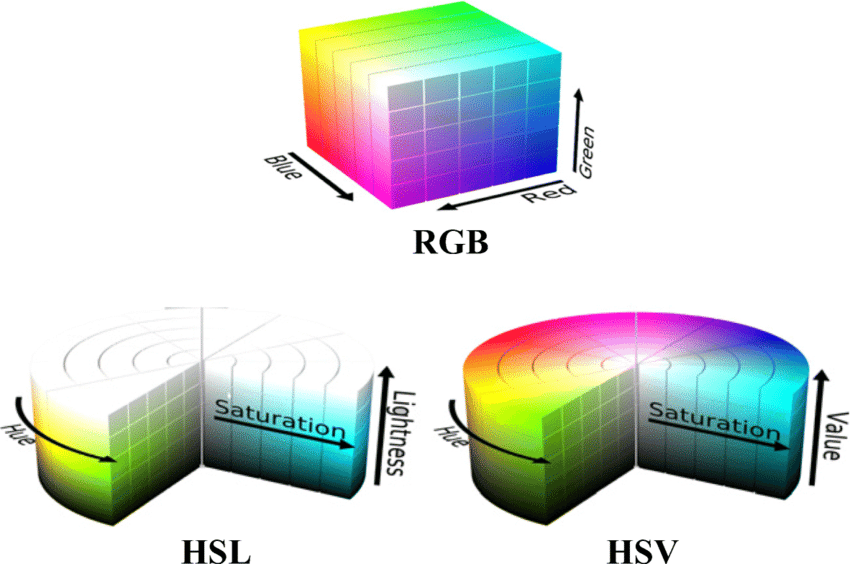
\includegraphics[width=0.6\textwidth]{figures/RBG_HSL_HSV}
	\fonte{\cite{rbg_hsl_hsv}}
	\label{rbg_hsl_hsv}
\end{figure}

\begin{figure}[ht]
	\centering
	\caption{Modelo HSV bidimensional}
	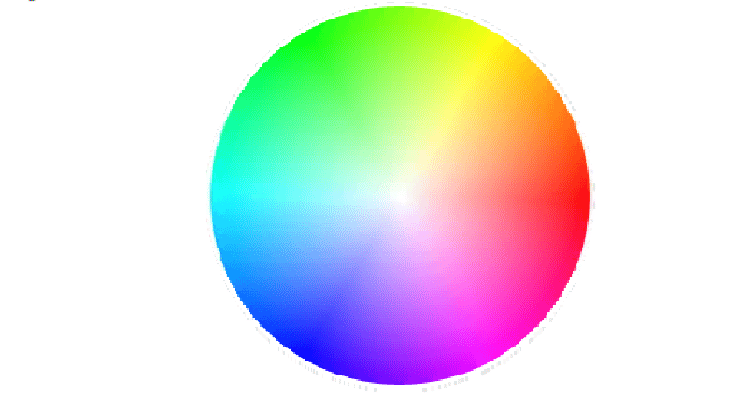
\includegraphics[width=0.8\textwidth]{figures/HSV}
	\fonte{ \cite{hsv_model}}
\end{figure}


O aplicativo retorna os valores em RGB, então usando um algorítimo
que converte RGB para HSV e invertendo o eixo Y
é possível ter os valores de angulo e módulo de um vetor velocidade.
A \autoref{hsv_exemplo_1} possue os valores RBG enviados pelo aplicativo
e a posição em que o cursor do aplicativo esta,
Esses valors, quando aplicados no algorítimo de conversão de RGB para HSV, geram os resultados na \autoref{HSV_resultado}
Facilmente podemos extrair informações de direção e magnitude que podem ser usados para controlar o robô.
Como mencionado anteriormente, o modelo HSV esta invertido no eixo Y,
então para obter o angulo representado pelo aplicativo, basta de 360 o subtrair o valor encontrado.

\begin{figure}[ht]
	\centering
	\caption{Aplicativo Android - Valores RGB e posição}
	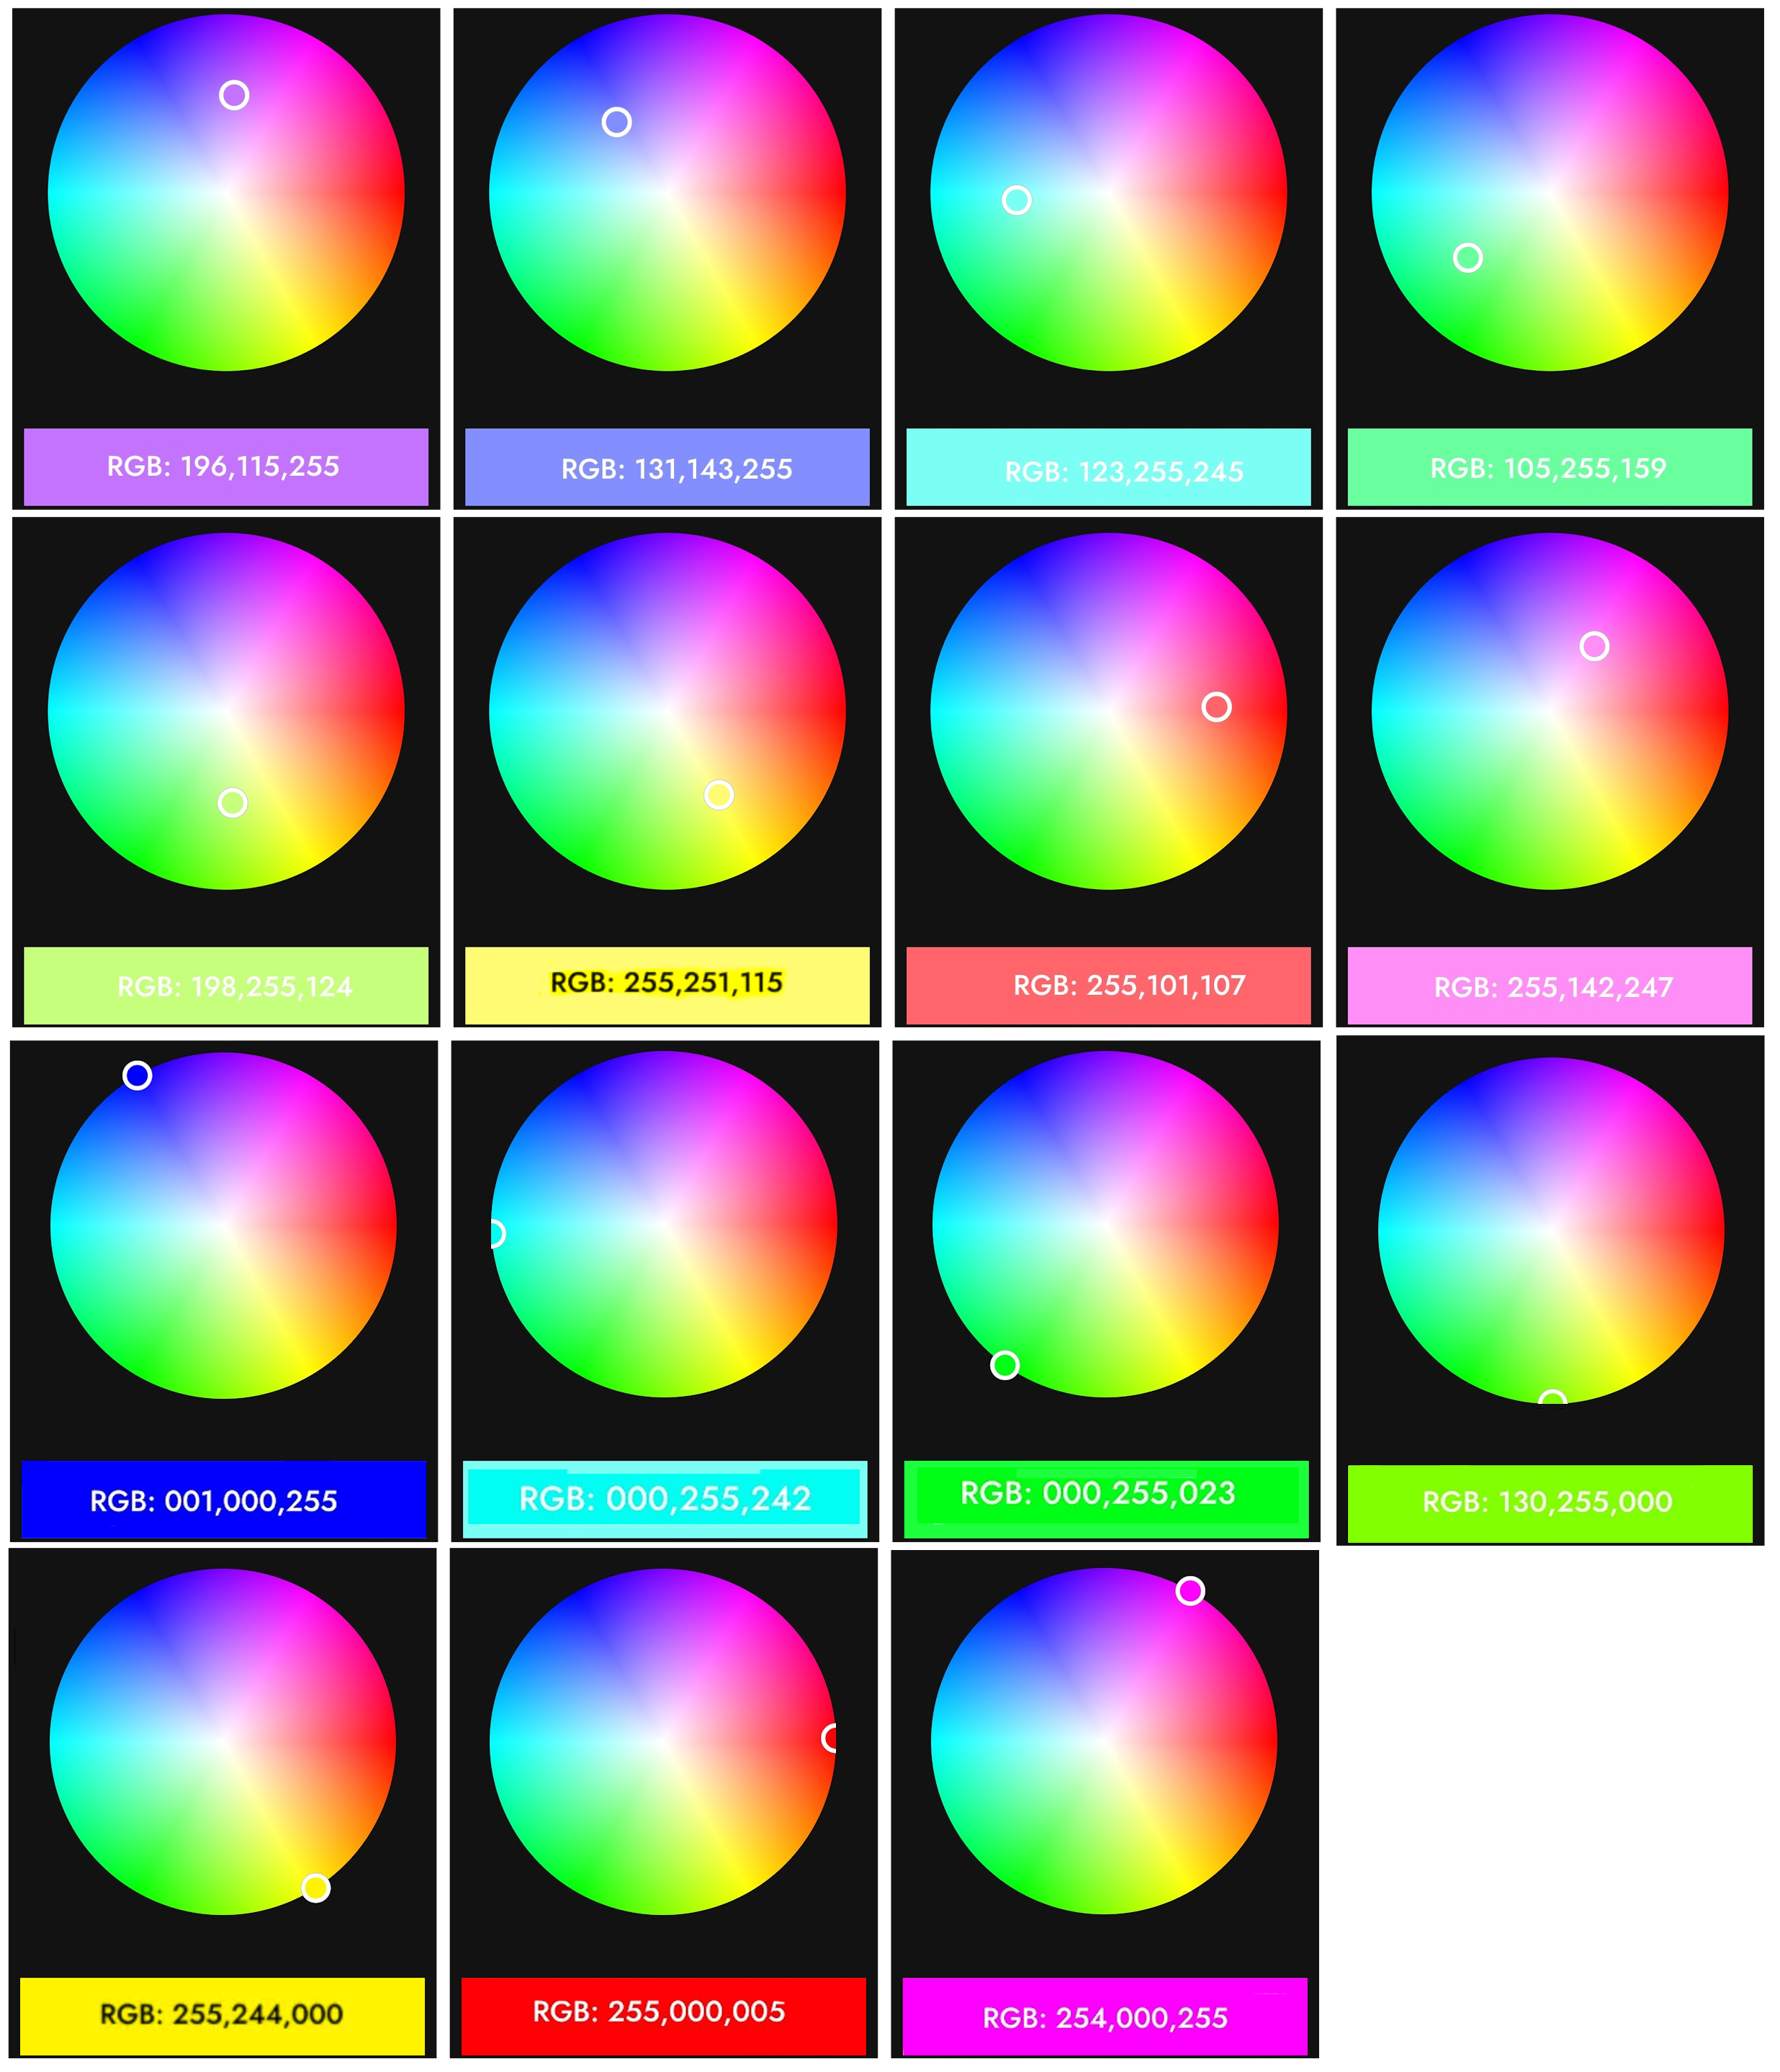
\includegraphics[width=1.0\textwidth]{figures/example_1_arduino_color}
	\fonte{Própria}
	\label{hsv_exemplo_1}
\end{figure}


\begin{table}[ht]
	\centering
	\caption{\label{HSV_resultado}Resultado do algoritmo de conversão de RGB para HSV}
	\begin{tabular}{|c|c|c|c|}
        \hline
        \textbf{RGB} & \textbf{Ângulo $\theta$} & \textbf{Magniture} & \textbf{Correção de ângulo (360-$\theta$)} \\ \hline
        196, 115, 255 & 275\textdegree & 54,9\% & 85\textdegree \\ \hline
        131, 143, 255 & 234\textdegree & 48,63\% & 126\textdegree \\ \hline
        123, 255, 245 & 175\textdegree & 51,76\% & 185\textdegree \\ \hline
        105, 255, 159 & 142\textdegree & 58,82\% & 218\textdegree \\ \hline
        198, 255, 124 & 86\textdegree & 51,37\% & 274\textdegree \\ \hline
        255, 251, 115 & 58\textdegree & 54,9\% & 302\textdegree \\ \hline
        255, 101, 107 & 358\textdegree & 60,39\% & 2\textdegree \\ \hline
        255, 142, 247 & 304\textdegree & 44,31\% & 56\textdegree \\ \hline
        001, 000, 255 & 240\textdegree & 100,0\% & 120\textdegree \\ \hline
        000, 255, 242 & 177\textdegree & 100,0\% & 183\textdegree \\ \hline
        000, 255, 023 & 125\textdegree & 100,0\% & 235\textdegree \\ \hline
        130, 255, 000 & 89\textdegree & 100,0\% & 271\textdegree \\ \hline
        255, 244, 000 & 57\textdegree & 100,0\% & 303\textdegree \\ \hline
        255, 000, 005 & 359\textdegree & 100,0\% & 1\textdegree \\ \hline
        254, 000, 255 & 300\textdegree & 100,0\% & 60\textdegree \\ \hline
	\end{tabular}
\end{table}

O algoritmo de conversão de RGB para HSV transtrito em C, pode ser encontrado no apêndice \ref{anx_rgb_to_hsv}.
É possível modificar o algoritmo para que o valor de magnitude seja mapeado em uma escala logaritma
para uma saida de velocidades maiores que zero de maineira mais suave,
e também é possível definir um diametro mínimo onde os valores
de magnitude seja sempre zero, dessa forma não é necessário muito
precisão do usuário para chegar em valores de zero.

\subsubsection{Demais controles}

Para demais ações e comandos para serem enviados para o microcontrolador
o aplicativo Serial Bluetooth Terminal permite enviar textos via terminal,
e atrelar textos predeterminados em botões de ação.

\begin{figure}[ht]
	\centering
	\caption{Tela do aplicativoSerial Bluetooth Terminal}
	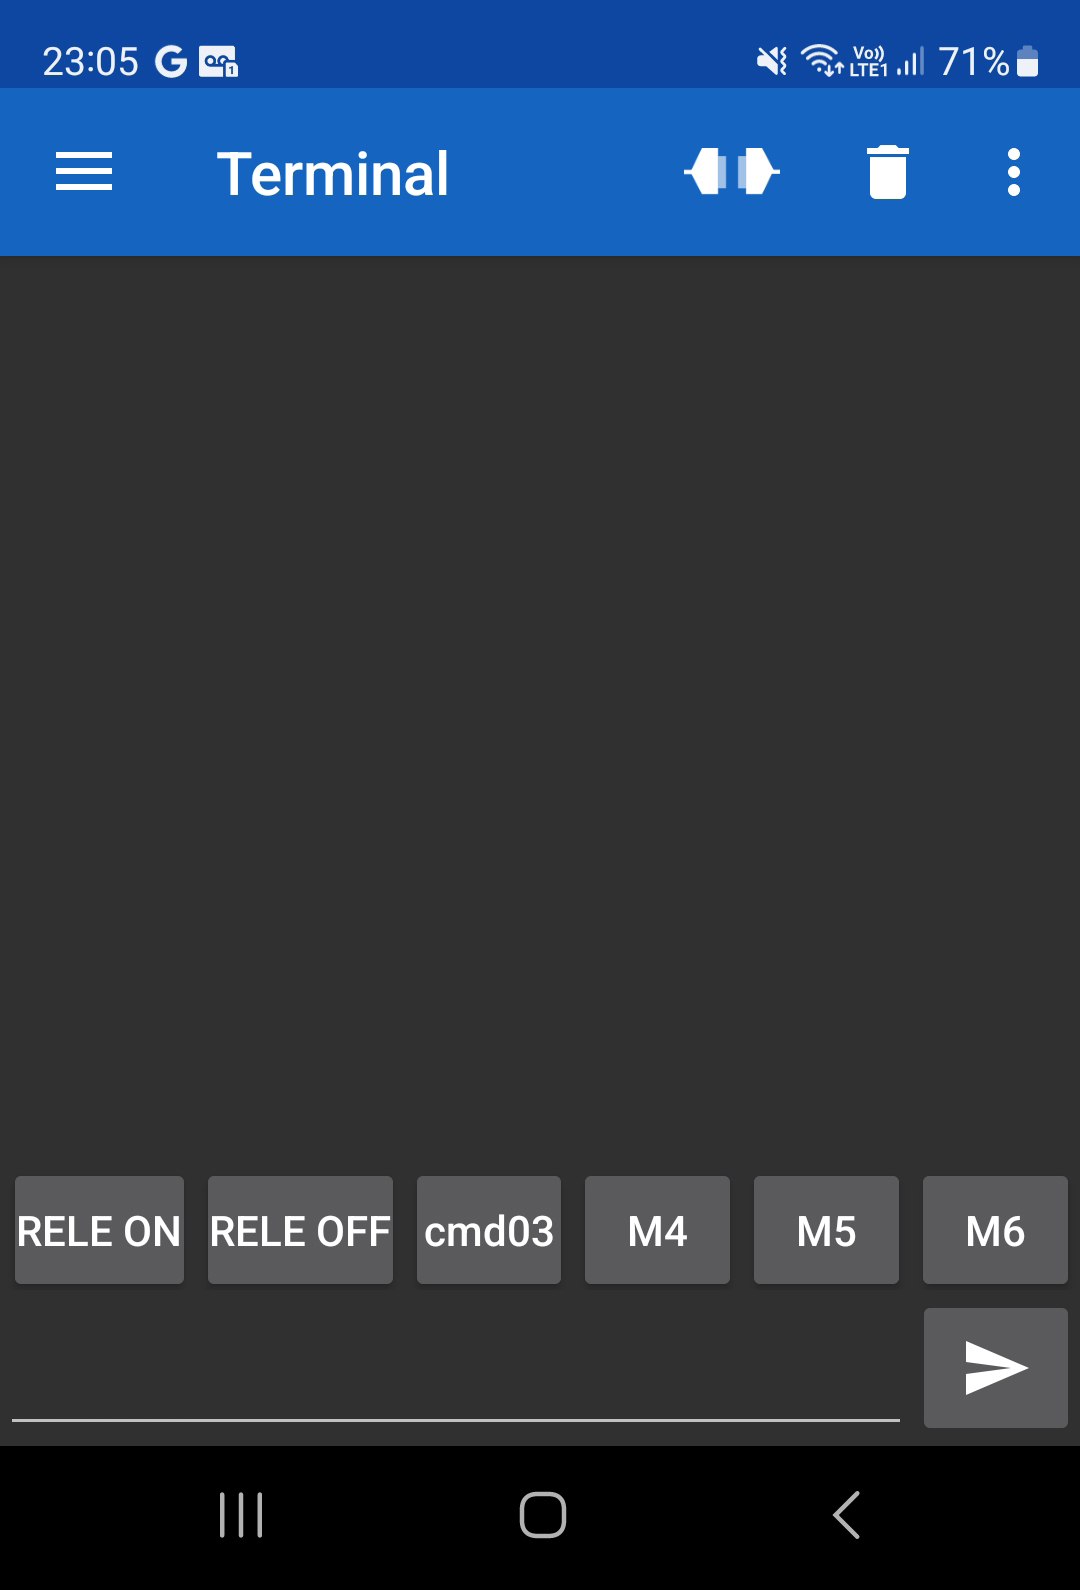
\includegraphics[width=0.40\textwidth]{figures/serialbluetoothterminal}
	\fonte{Própria}
	\label{serialbluetoothterminal_tela}
\end{figure}


\section{Alimentação}


\subsection{Microcontrolador}

Para alimentação do ESP32, pode usar tanto uma bateria de 5v ou 3.3v, pois possui dois pinos para alimentação: 

\subsubsubsection{Pino de 5v não regulado}

Fontes divergem em relação à tensão máxima (\cite{esp32_reference_power_supply_1}, \cite{esp32_reference_power_supply_2}),
que pode ser usada, porém, a maioria concorda em manter de 6v a 7v.

\subsubsubsection{Pino de 3.3v regulado}
Esse pino pode receber no máximo 3.3v, podendo funcionar entre 3.1v e 3.3v sem problema.

\subsubsubsection{micro USB}
Essa opção permite usar um powerbank, porém o conector do ESP32 é um Micro-USB B, modelo que usa protocolo USB 2.0, que pode fornece apenas a 500mA a 5v \cite{micro_usb_b}.
500mA É suficiente para alimentar o ESP32, que pode consumir até 260mA \cite{esp_max_current}.
Porem um powerbank pode ser uma solução muito ineficiente do ponto de vista energético, os modelos populares possuem baterias de lítio de 3.7v, que é convertido para 5v,
e posteriormente dentro do ESP32 a tensão é convertida novamente para 3.3v. Apenas no modelo PN-952 da CNHPineng sai de 5000mAh a 3.7v  para 3160mAh a 5v,
podendo novamente perder mais corrente por hora ao ser convertido para 3.3v no ESP32


\subsection{Motores DC}
\lipsum[1]

\subsection{Motores de passo}

Os motores de passo NEMA 17 podem ser alimentados, através do driver, com 12v a 24v.
Observando a possibilidade de uma bateria de 12v/24v ficar sem uso depois do projeto,
e considerando que ferramentas elétricas possuem baterias padronizadas de 12v/18v/36V, foi considerando utilizar 3 baterias de 12v da bosch, que já estavam disponíveis para uso.
Cada bateria tem tensão nominal de 12v a 2Ah, do modelo GBA, que são usadas em aspirador de pó, esmerilhadeiras, furadeiras, plainas e serras circulares.



\section{Motores}  \label{secao_motores}

\subsection{Motores DC}


Um motor DC é essencialmente uma máquina elétrica de corrente contínua, que
converte energia elétrica de corrente contínua em energia mecânica. Máquinas
elétricas de corrente contínua são mais fácies de se controlar (quando
comparadas a máquinas de corrente alternada) e oferecem uma grande faixa de
velocidades \cite{Maquinas_eletricas}. Devido a essas características, tornam-se
boas candidatas para uso em eletrônica e robótica, uma vez que é viável
utilizá-las com com baterias. Para controlar a velocidade de um motor, é
necessário o uso de um encoder, que converte o sinal de posição em um valor
mensurável de velocidade angular, e também um driver, que permite a
microcontroladores controlarem a atuação do motor.

\subsubsection{Encoder magnético}

	Encoders magnéticos são um tipo de encoder rotacional que utiliza sensores 
	para identificar alterações em campos magnéticos a partir de uma roda ou 
	anel magnéticos. A rotação detectada é expressa em termos de pulsos de maior
	ou menor duração, a depender da resolução do encoder. Um encoder incremental
	mede a posição relativa do eixo (em contraste com encoders absolutos), em
	incrementos, a partir de dois sensores magnéticos, indicando a quantidade de
	pulsos percorridos entre a posição de referência e a posição atual.
	
	Há alguns tipos diferentes de se medir e representar a resolução de um
	encoder magnético. Na representação de pulsos por revolução (PPR), o valor 
	apresentado descreve o número de pulsos em valor alto que um encoder terá em
	qualquer uma das suas duas saídas quadráticas. Uma outra representação comum
	de resolução de encoders é CPR (contagens por revolução), que representa o
	número de estados de quadratura decodificados que existem entre as duas
	saídas do encoder (representando, portanto, o valor de uma resolução dada em
	PPR multiplicada por 4). Outras formas de representar a resolução de um
	encoder são LPR (linhas por revolução, referindo-se a às barras marcadas no
	disco óptico de um encoder, cada uma representando um pulso de valor baixo),
	e também ciclos por revolução (cujo acrônimo ocasionalmente é dado também
	como CPR por fabricantes) - o valor apresentado em ambas as representações 
	equivale à representação em PPR (que é a representação adotada para
	avaliação e apresentação dos componentes utilizados neste trabalho). 
	
	Em encoders magnéticos incrementais, são produzidas duas ondas quadradas
	como saídas, A e B \cite{encoder_ppr}. As duas possuem 90° de fase entre si,
	e, caso a onda A esteja adiantada em relação a B (\autoref{encoder_ppr_ab}),
	o sentido de rotação é positivo (anti-horário).

\begin{figure}[ht]
	\centering
	\caption{Encoder holzer}
	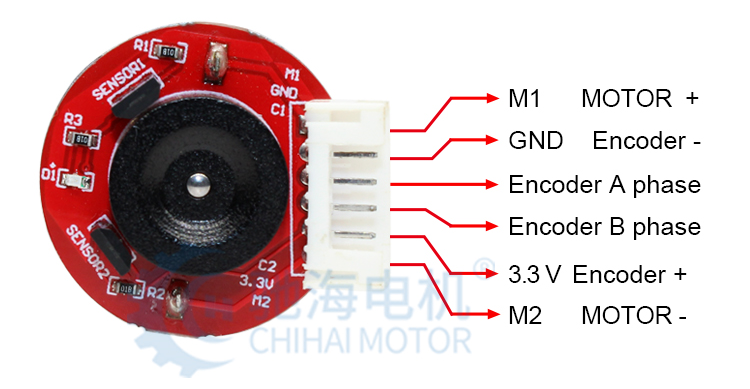
\includegraphics[width=0.6\textwidth]{figures/encoder_holzer}
	\caption{FONTE: \cite{motor_dc_6v_encoder}}
\end{figure}

\begin{figure}[ht]
	\centering
	\caption{Ondas quadradas resultantes dos pulsos de saída do encoder}
	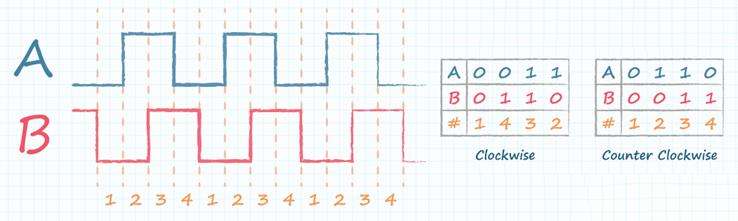
\includegraphics[width=0.6\textwidth]{figures/encoder_pulso_ab}
	\caption{FONTE: \cite{encoder_ppr}}
	\label{encoder_ppr_ab}
\end{figure}


\subsubsection{Motor DC e encoder}
Para a versão inicial do robô, foi decidido trabalhar com motor DC.
Motores DC são mais difíceis de controlar que motores de passo, porém tem uma resposta mais rápida, e se o controle for
bem aplicado, podem ter também um melhor desempenho. A complexidade do controle de um motor DC apresenta um bom desafio
para aplicação dos conceitos e disciplinas do curso de Engenharia de Instrumental, Automação e Robótica. O motor DC 
escolhido foi um de 6V 210rpm, com taxa de redução de 1:34. Tal motor já possui um encoder magnético acoplado, com 11
PPR (\textit{"Pulses Per Revolution"}), resultando em um encoder com resolução de 374 PPR.

\begin{figure}[htb]
	\centering
	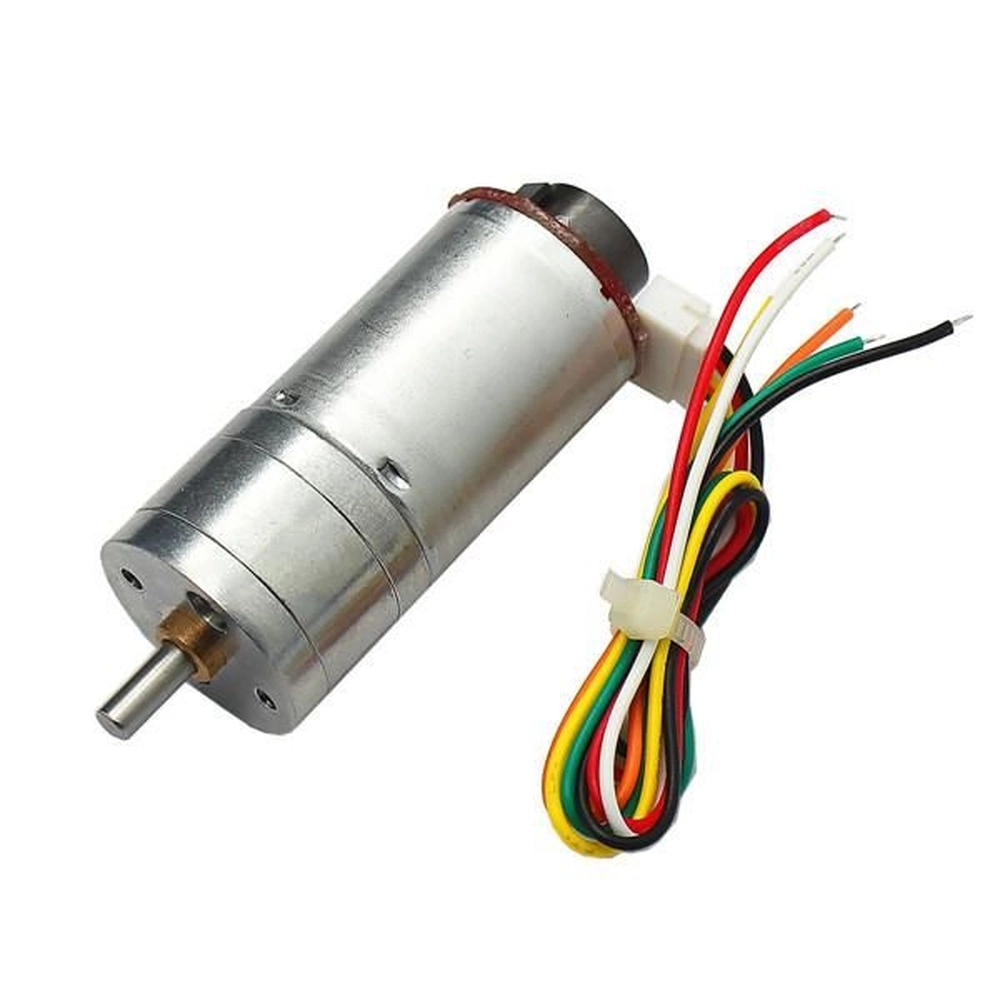
\includegraphics[width=0.7\textwidth]{figures/CHR_GM25_370}
	\caption{Motor DC 6V \cite{motor_dc_6v_encoder}}
\end{figure}

\begin{quadro}[htb]
\caption{\label{Especificacoes_motordc_6v}Especificações do motor DC 6V}
	 \begin{tabular}{|c|c|c|c|}
		\hline
		\textbf{Especificação} & \textbf{Valor} \\ \hline
		Tensão nominal & DC 6V  \\ \hline
		Velocidade sem carga  & 210RPM 0.13A  \\ \hline
		Eficiência máxima & 2,0kg.cm/170rpm/2,0W/0,60A   \\ \hline
		Poder máximo & 5,2kg.cm/110rpm/3,1W/1,10A   \\ \hline
		Torque de parada  & 10kg.cm 3.2A    \\ \hline
		Taxa de Redução do Retardador & 1:34  \\ \hline
		Resolução do salão & Razão Hall x 34,02 = 341,2PPR  \\ \hline
	\end{tabular}
	\fonte{\cite{chinhai_motor}}
\end{quadro}


\subsubsection{Driver de Motor}
Nas etapas iniciais do projeto, testou-se driver Ponte H L298N para ligar cada motor. Esse driver suporta até 2A em
operação DC \cite{datasheel_l298n}. A corrente de operação máxima do motor é de 1.1A; contudo, a corrente de parada
pode chegar a 3.2A. Além disso, o L298N também causa uma queda de tensão significativa: a uma corrente de 1A, a queda
observada chegou a até 3.2V, fazendo com que o motor não receba a tensão necessária para operar nas condições
desejadas \cite{datasheel_l298n}. As observações são compatíveis com as expectativas de faixa de operação do L298N - a
seu uso é recomendado para tensões entre 12V a 40V, em que a queda de tensão observada não seja tão significativa
relativamente. Devido à natureza da aplicação deste projeto, com o motor de 6v, a queda de tensão acaba sendo
intolerável, inviabilizando assim o uso da ponte H L298N.

Após essas considerações e observações, optou-se por um driver apropriado para uso em baixas tensões, o DRV8833
\cite{datasheel_dvr8833}.


\subsection{Controle de velocidade}

\subsubsection{Medição de velicidade do motor}

Como encoder possuí dois sinais de onda quadadra defasadas em 90º, fase A e fase B, cujos vales e picos são valores lógicos HIGH e LOW, 
e direção de rotação do motor pode ser definida pela diferença entre as fases, se fase A esta adiantada ou atrasada em relação a fase B
É possível calcular a velocidade com base nas subidas da onda quadrada de uma fase, e o valor logico da outra fase no momento da subida.
Por exemplo,  observando a fase B, toda vez em que há uma subida, se o valor da fase A for alto, então incrementar +1 em um contador, se a fase A tiver valor baixo, então incrementar -1 no contador.
Quando o valor da fase A for alto, então o motor esta rodando em um sentido,  quando o valor  for baixo, então o motor esta rodando no sentido contrário.
Medindo o valor do contador por um $\Delta_{T}$, se resulta na quantidade de pulsos por segundo.
Para converter de pulsos por segundo para RPM, basta dividir pela resolução do motor+encoder,  que é de 1:34 do motor, e 11 pulsos por rotação do encoder, o que resulta em 374,
e multiplicar por 60 para ter o resultado em rotações por minuto.

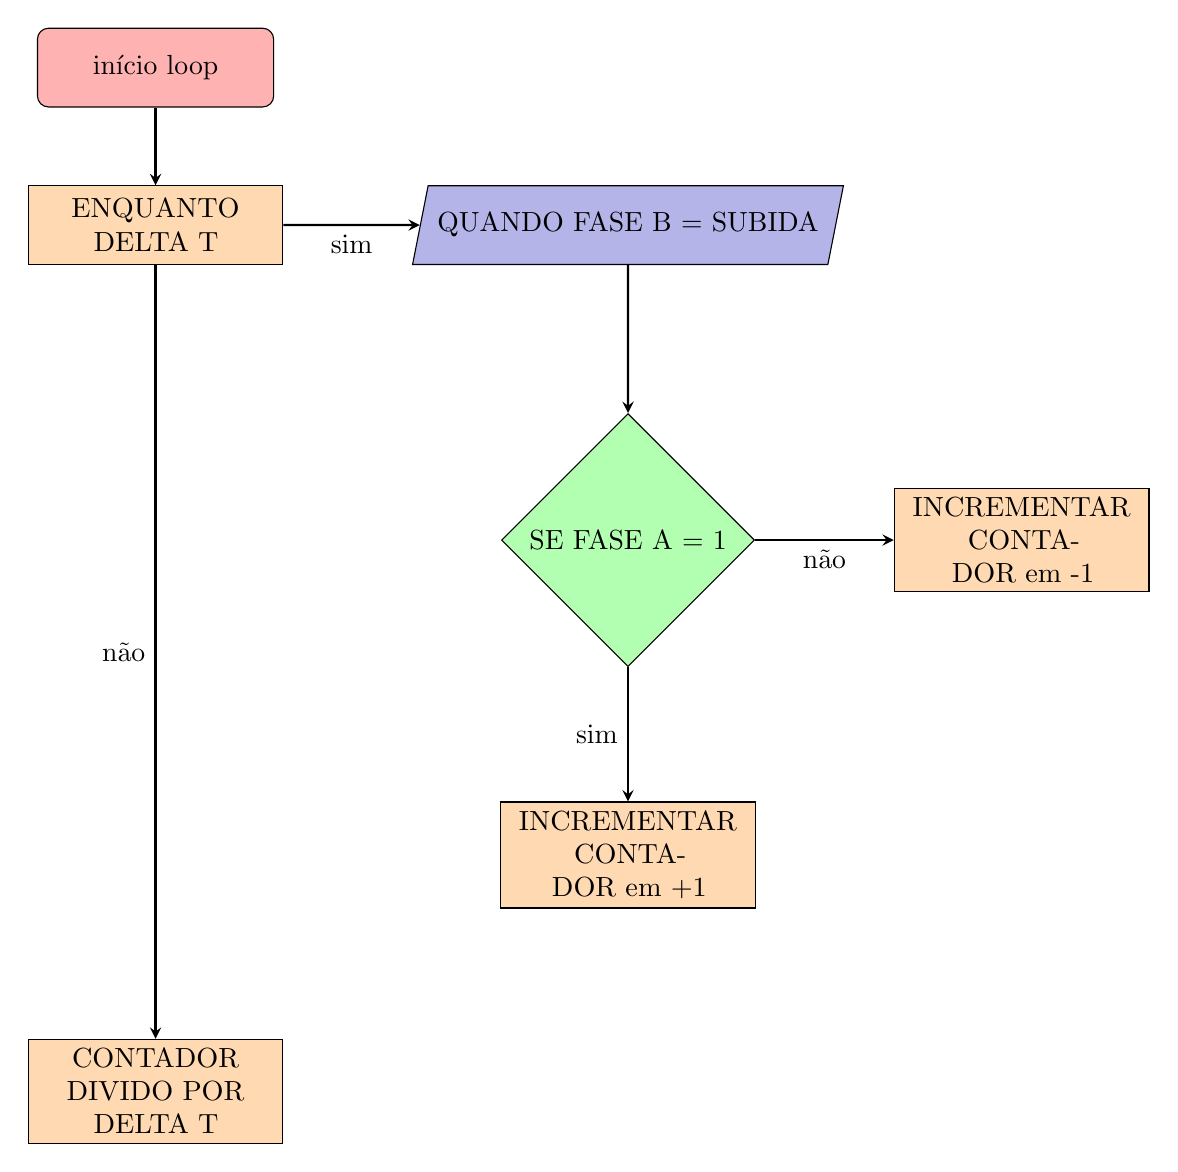
\begin{tikzpicture}[node distance=2cm]

    \node (start) [startstop] {início loop};
    \node (pro1) [process, below of=start] {ENQUANTO DELTA T};
    
    \node (in1) [io, right of=pro1, xshift= 4cm] {QUANDO FASE B = SUBIDA};
    
    \node (dec1) [decision, below of=in1, yshift=-2cm] {SE FASE A = 1};
    \node (pro1a) [process, below of=dec1, yshift= -2cm] {INCREMENTAR CONTADOR em +1};
    \node (pro1b) [process, right of=dec1, xshift= 3cm] {INCREMENTAR CONTADOR em -1};
    
    
    \node (count) [process, below of=pro1, yshift= -9cm] {CONTADOR DIVIDO POR DELTA T};
    
    \draw [arrow] (start) -- (pro1);
    \draw [arrow] (pro1) -- node[anchor=north] {sim} (in1);
    \draw [arrow] (in1) -- (dec1);
    \draw [arrow] (dec1) -- node[anchor=east] {sim} (pro1a);
    \draw [arrow] (dec1) -- node[anchor=north] {não} (pro1b);
    
    \draw [arrow] (pro1) -- node[anchor=east] {não} (count);

\end{tikzpicture}



Na implementação dessa lógica no STM32, o desafio foi a definição do $\Delta_{T}$,
Se o $\Delta_{T}$ for muito pequeno, o resultados de pulsos por segundo pode tender ao infinito, gerando valores muito altos.
Na figura \ref{fig:medidas_altas} em laranja, esta o resultado do rpm considerando o $\Delta_{T}$ como o tempo entre os ciclos do micrcontrolador.
A outra opção, foi definir um $\Delta_{T}$ fixo, definindo uma frequencia de medição pré definida, e o resultado pode ser visto em azul na figura \ref{fig:medidas_altas}
Essa outra opção de $\Delta_{T}$ resultou em um sinal que tem uma componente em alta frequência com uma amplitude até consideral.
Analisando os dois sinais no dominio da frequêcia na figura \ref{fig:frequencia_medidas_altas}, o espectro em frequência do sinal em laranja possui amplitudes muitos semelhante em todo espectro, mas o espectro do sinal em azul, fica bem claro que em altas frequencias é composto mais por ruidos
e as frequencia médias tem amplitude menor em relação as frequências baixas, o que torna mais fácil aplicar um filtro passa-baixa para reduzir as frenquências médias e altas.

A figura \autoref{passa_baixa_teste}, mostra um dos teste de filtro passa baixa, em o sinal em laranja ainda persiste esses valores tentendo ao infinito, devido a ampliture eles se tornam um pouco dificil de serem retirados.
Mas o sinal em azul acaba tendo um resultado melhor depois do filtro, muito semelhando ao sinal em laranja.
Com base nesse resultado, foi decidido seguir com o método em que o $\Delta_{T}$ é definido por uma frequência pré definida.


\begin{figure}[h]
    \centering
    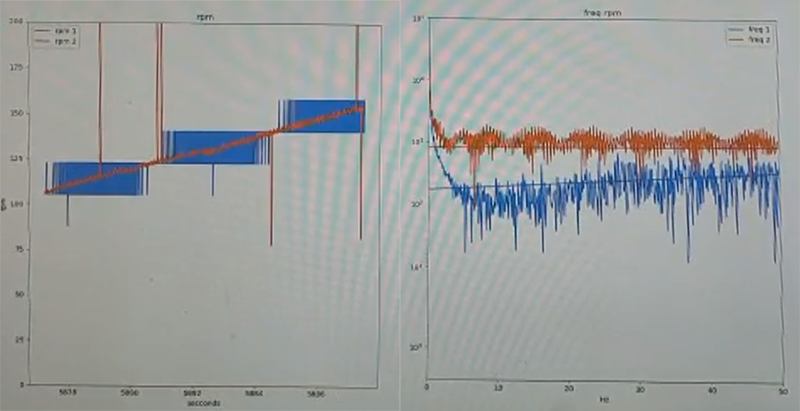
\includegraphics{figures/medidas_altas}
    \caption{Problemas com delta T muito pequeno}
    \label{fig:medidas_altas}
\end{figure}

\begin{figure}[h]
    \centering
    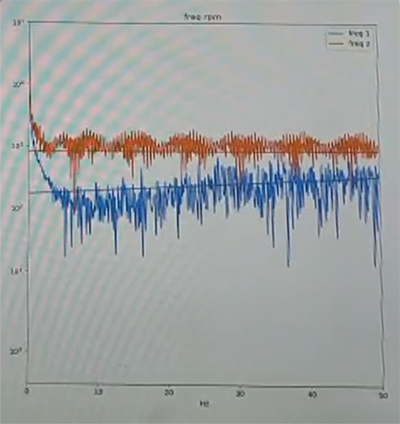
\includegraphics{figures/frequencia_medidas_altas}
    \caption{Frequências}
    \label{fig:frequencia_medidas_altas}
\end{figure}

\begin{figure}[h]
    \centering
    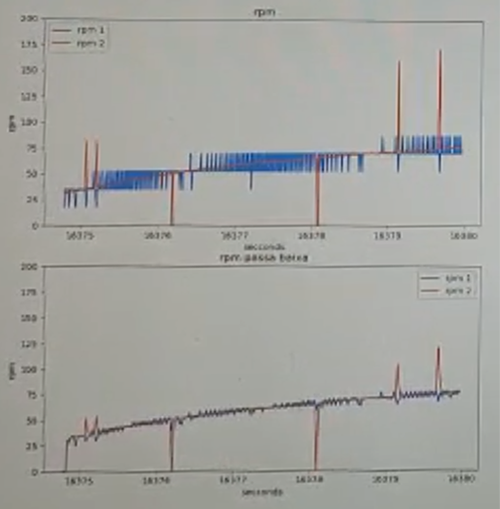
\includegraphics{figures/passa_baixa_teste}
    \caption{Passa baixa teste}
    \label{fig:passa_baixa_teste}
\end{figure}


Com o método definido, foi definido um $\Delta_{T}$ em 100hz eu um filtro passa baixa em 2hz
As imagens no anexo \autoref{att_medicao_motores}, mostra as imagens comparando o sinal original e o sinal filtrado para cada motor.
A equação \autoref{eqn:equacao_diferenca} a seguir é a equação de diferença do filtro, considerando uma amostragem de 100hz e frequência de corte em 2hz.

\begin{equation}
    \begin{split}
        y[k] = 0.0591174 \cdot u \left[ k \right] +  0.0591174 \cdot u[k - 1] + 0.88176521 \cdot y[k - 1]
    \end{split}
    \label{eqn:equacao_diferenca}
\end{equation}

\subsubsection{Curva PWM x RPM - problema da não linearidade}

Depois de definido como calcular a velocidade o próximo desafio foi lidar com a não linearidade entre o PWM e o resultado medido em RPM.
Como pode ser visto na figura \autoref{grafico_pwm_x_rpm}, na comparação entre o valor do PWM e o RPM no tempo.

\begin{figure}[htb]
	\centering
	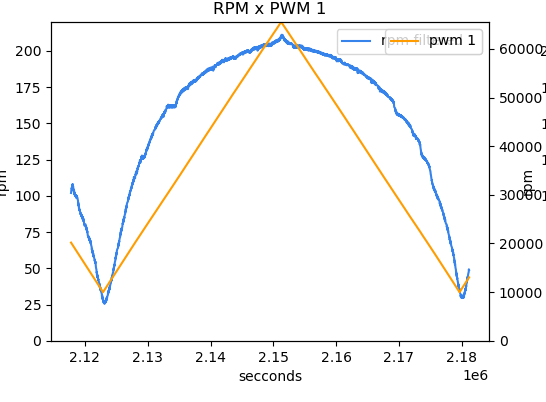
\includegraphics{figures/pwm_x_rpm}
	\caption{Curva PWM e RPM no tempo}
	\label{fig:grafico_pwm_x_rpm}
\end{figure}

Considerando essa não linearidade, foram realizadas 15k medições em PWM vs RPM para definir uma equação que pudesse relacionar o PWM com o RPM.
Como pode ser observado na figura  \autoref{medicao_pwm_x_rpm_dados_brutos}, os resultados possuem uma tendência, mas possuem alguns pontos fora da curta.
devido ao esses ruídos nas medições ss dados foram tratatos para obter valores médios dos resultados usando python,
o código pode ser visto no anexo \autoref{att_limpeza_python}.

\begin{figure}[htb]
	\centering
	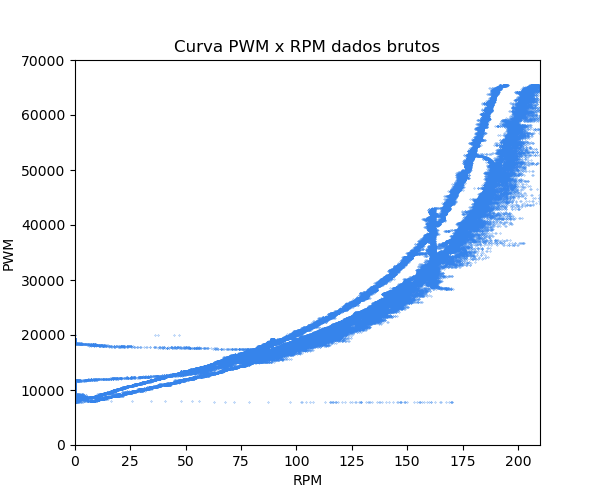
\includegraphics{figures/curva_pwm_x_rpm_dados_brutos}
	\caption{Curva PWM x RPM dados brutos}
	\label{fig:medicao_pwm_x_rpm_dados_brutos}
\end{figure}


O resultado da limpeza dos dados pode ser vizualizado na figura \autoref{medicao_pwm_x_rpm_dados_medios}.
Após a limpeza dos dados, os dados foram importados para o matlab, anexo \autoref{att_matlab},
para obter um polinômio que possa definir a curva, o polinômio resultante é a equação \ref{eqn:polimonio_rpm}, e a figura \autoref{curva_ajustada} representa a curva ajustada.
A equação do polinômio foi inserida no código do micrcontrolador, foi testado definir um RPM de 150, e a tabela \autoref{medicao_motores} trás uma amostra dos resultados dos RPMs de cada motor.
Com essa equação é mais fácil definir um comportamento linear, facilitando a aplicação de um controle PDI.

\begin{equation}
    \begin{split}
        0.0001131x^{4} + -0.03064x^{3} + 2.993x^{2} + -1.257x + 9017
    \end{split}
    \label{eqn:polimonio_rpm}
\end{equation}

\begin{figure}[htb]
	\centering
	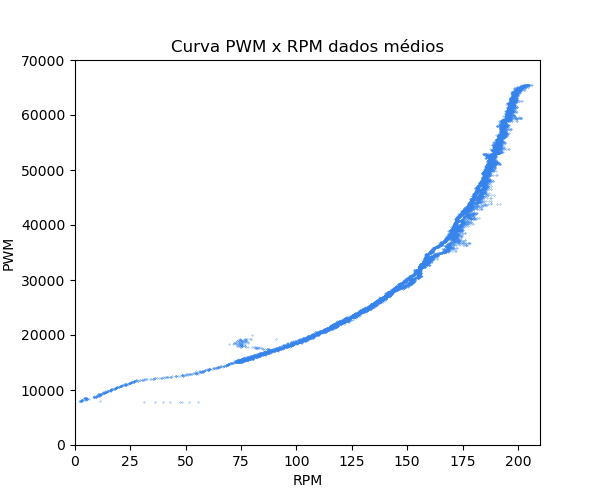
\includegraphics{figures/curva_pwm_x_rpm_dados_medios}
	\caption{Curva PWM x RPM dados médios}
	\label{fig:medicao_pwm_x_rpm_dados_medios}
\end{figure}

\begin{figure}[htb]
	\centering
	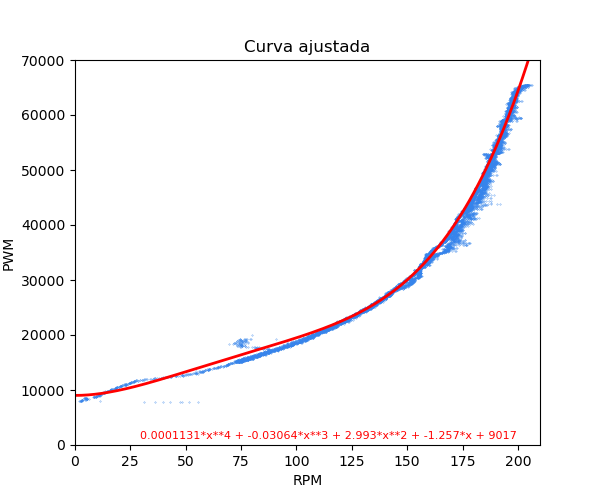
\includegraphics{figures/curva_ajustada}
	\caption{Curva ajustada}
	\label{fig:curva_ajustada}
\end{figure}



\begin{quadro}[htb]
	\caption{\label{medicao_motores}Medição rpms motores}
	 \begin{tabular}{|c|c|c|c|c|}
		\hline
		\textbf{$Tempo_{seg}$} & \textbf{$RPM_{definido}$} & \textbf{$RPM_{real_{1}}$} & \textbf{$RPM_{real_{2}}$} & \textbf{$RPM_{real_{3}}$} \\ \hline
		52.954 & 150.00  & 141.03 & 162.69 & 149.82 \\ \hline
		52.954 & 150.00  & 141.43 & 162.43 & 149.18 \\ \hline
		53.000 & 150.00  & 140.83 & 162.19 & 148.61 \\ \hline
		53.000 & 150.00  & 140.30 & 161.98 & 149.06 \\ \hline
		53.000 & 150.00  & 140.79 & 161.80 & 149.46 \\ \hline
		53.000 & 150.00  & 141.21 & 161.64 & 148.86 \\ \hline
		53.046 & 150.00  & 141.59 & 161.49 & 149.28 \\ \hline
		53.046 & 150.00  & 141.92 & 161.37 & 149.65 \\ \hline
		53.046 & 150.00  & 141.26 & 161.25 & 149.02 \\ \hline
		53.046 & 150.00  & 140.68 & 162.11 & 148.48 \\ \hline
		53.046 & 150.00  & 141.12 & 162.86 & 148.94 \\ \hline
		53.092 & 150.00  & 141.51 & 162.57 & 149.35 \\ \hline
		53.092 & 150.00  & 141.85 & 162.32 & 148.76 \\ \hline
		53.092 & 150.00  & 141.20 & 162.09 & 149.19 \\ \hline
		53.092 & 150.00  & 140.63 & 161.90 & 149.57 \\ \hline
	\end{tabular}
\end{quadro}


\subsection{Implementação da medição de rpm e filtro passa baixa no microcontrolador}

Para medir a velocidade de um motor DC com base no encoder, foi necessário realizar a leitura das subidas dos calores de LOW para HIGH de uma das fases do enconder, e comparar com outra Fase
Para isso usamos o sistema de interrupção do microcontrolador.
Exemplo do trecho de código que realiza a leitura dos valores do encoder, e registra em um contador a quantidade de pulsos de uma fase.


\lstset{language=C}
\begin{lstlisting}
long prevTime = 0;
long currTime = micros();
volatile int pos_i_1 = 0;
int prevPosition_1 = 0;
void setup() {
    motorsSetupPins(); encodersSetupPins();
    attachInterrupt(digitalPinToInterrupt(PB0), readEncoder1, RISING);
}
void loop() {
	int currPosition_1 = 0;
    ATOMIC_BLOCK(ATOMIC_RESTORESTATE){currPosition_1 = pos_i_1;};
    prevPosition_1 = currPosition_1;
}

void readEncoder1(){ 
    int b = digitalRead(PB1);
    if(b>0){pos_i_1++;}
    else {pos_i_1--;}
}
\end{lstlisting}


Após obtendo os a quantidade de pulsos é possivel calcular a taxa de pulsos por segundo, usando o diferencial da velocidade no dominio discreto, $\Delta$p/$\Delta$t.

\lstset{language=C}
\begin{lstlisting}
#define HALL_RESOLUTION 374
long prevTime = 0;
long currTime = micros();
volatile int pos_i_1 = 0;
int prevPosition_1 = 0;
float direction_angle = 90;
void setup() {
    motorsSetupPins();
    encodersSetupPins();
    attachInterrupt(digitalPinToInterrupt(PB0), readEncoder1, RISING);  
}
void loop() {
	currTime = micros();
	int currPosition_1 = 0;
	ATOMIC_BLOCK(ATOMIC_RESTORESTATE){currPosition_1 = pos_i_1;};
	float rpm1 = calc_rpm(currTime, prevTime, currPosition_1, prevPosition_1);
	prevPosition_1 = currPosition_1;
	prevPosition_3 = currPosition_3;
	prevTime = currTime;
}
void readEncoder1(){ 
    int b = digitalRead(PB1);
    if(b>0){pos_i_1++;}
    else {pos_i_1--;}
}
float calc_rpm(long currT, long prevT, int pos, int posPrev){
    float deltaT = ((float) (currT-prevT))/1.0e6;
    float pulse_per_seconds = (pos - posPrev)/deltaT;
    float rpm = 60*pulse_per_seconds/HALL_RESOLUTION;
    return rpm;
}
\end{lstlisting}


Porém calcular velocidade a cada ciclo do micrcontrolador acaba registrando valores de tempo muito pequenos, fazendo a velocidade tender ao infinito
A solução foi estabelecer uma amostragem do registro da velocidade, porem a amostragem adiciona um ruido com frequências maiories que do sinal original e de amplitude definida.
Para retirar essas frequência do sinal, o filtro passa baixa foi implementado no código.


\lstset{language=C}
\begin{lstlisting}
#define HALL_RESOLUTION 374
#define DT_TIME_SAMPLE_RATE_ENCODER 10 // encoder position reading update rate
int nextChangeSampleRate  = (millis() + DT_TIME_SAMPLE_RATE_ENCODER);
long prevTime = 0;
long currTime = micros();
volatile int pos_i_1 = 0;
int prevPosition_1 = 0;
float filterRpm_1 = 0;
float prevRpm_1 = 0;
void setup() {
    encodersSetupPins();
    attachInterrupt(digitalPinToInterrupt(PB0), readEncoder1, RISING);   
}

void loop() {
    if (millis()>=nextChangeSampleRate){
        currTime = micros();
        int currPosition_1 = 0;
        ATOMIC_BLOCK(ATOMIC_RESTORESTATE){currPosition_1 = pos_i_1;};
        float rpm1 = calc_rpm(currTime, prevTime, currPosition_1, prevPosition_1);
        filterRpm_1 = low_pass_filter_first_order(rpm1, prevRpm_1, filterRpm_1);
        prevPosition_1 = currPosition_1;
        prevRpm_1 = rpm1;
        prevTime = currTime;
        nextChangeSampleRate = millis() + DT_TIME_SAMPLE_RATE_ENCODER;
    }
}
void readEncoder1(){ 
    int b = digitalRead(PB1);
    if(b>0){pos_i_1++;}
    else {pos_i_1--;}
}
float calc_rpm(long currT, long prevT, int pos, int posPrev){
    float deltaT = ((float) (currT-prevT))/1.0e6;
    float pulse_per_seconds = (pos - posPrev)/deltaT;
    float rpm = 60*pulse_per_seconds/HALL_RESOLUTION;
    return rpm;
}
float low_pass_filter_first_order(float currRpm, float prevRpm, float prevFilterRpm){
    float posFilterRpm = 0.881765*prevFilterRpm + 0.0591174*currRpm + 0.0591174*prevRpm;
    return posFilterRpm;
}
\end{lstlisting}

\subsection{Motores de passo}

\lipsum[1]




%https://www.aarohies.com/what-is-the-difference-between-pmdc-bldc-and-pmsm-motor/
%https://www.monolithicpower.com/en/learning/resources/brushless-vs-brushed-dc-motors
%https://techweb.rohm.com/product/motor/brushed-motor/209/

\section{dummy 1}

\lipsum[1]
\chapter{Fabricação e montagem - CAD}
\label{att_fabricao_montagem_cad}

\begin{figure}[h]
	\centering
	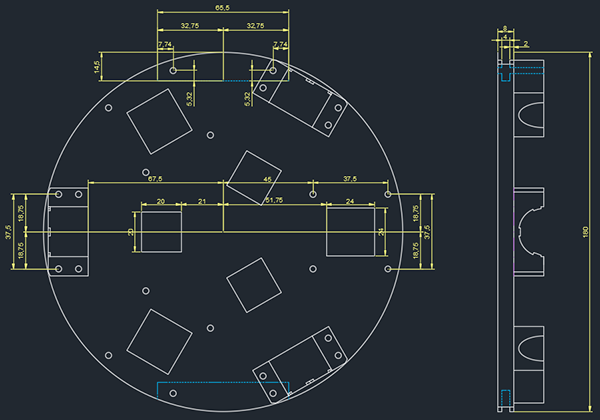
\includegraphics{figures/cad1}
	\caption{Base do robô}
	\label{fig:base_robo}
\end{figure}

\begin{figure}[h]
	\centering
	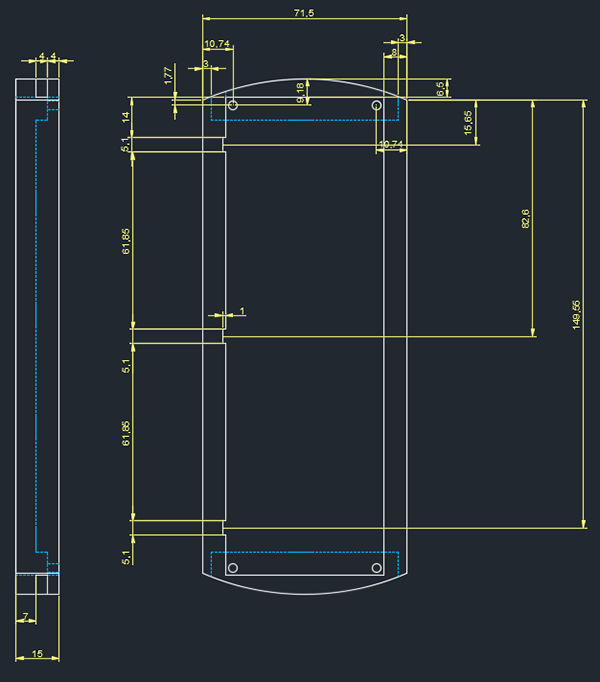
\includegraphics{figures/cad2}
	\caption{Suporte Protoboard}
	\label{fig:suport_protoboard}
\end{figure}

\begin{figure}[h]
	\centering
	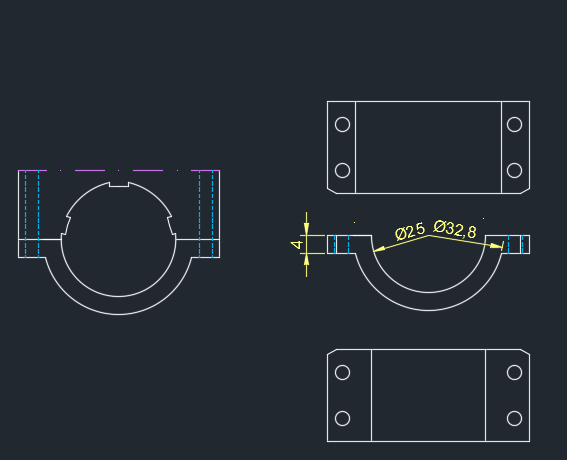
\includegraphics{figures/cad3}
	\caption{Abraçadeira dos Motores - 1}
	\label{fig:abracadeira}
\end{figure}

\begin{figure}[h]
	\centering
	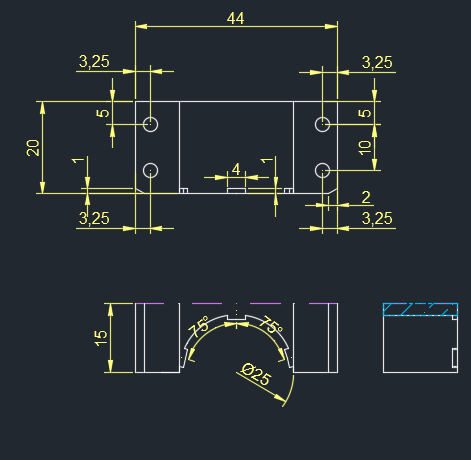
\includegraphics{figures/cad3_2}
	\caption{Abraçadeira dos Motores - 2}
	\label{fig:abracadeira_2}
\end{figure}

\begin{figure}[h]
	\centering
	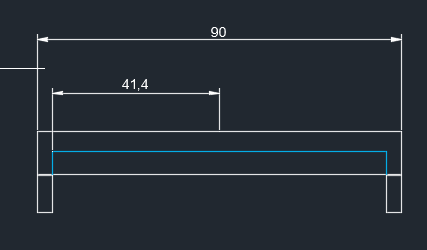
\includegraphics{figures/cad4}
	\caption{peça que conecta o suporte de protoboard e a base - 1}
	\label{fig:peca_juncao}
\end{figure}

\begin{figure}[h]
	\centering
	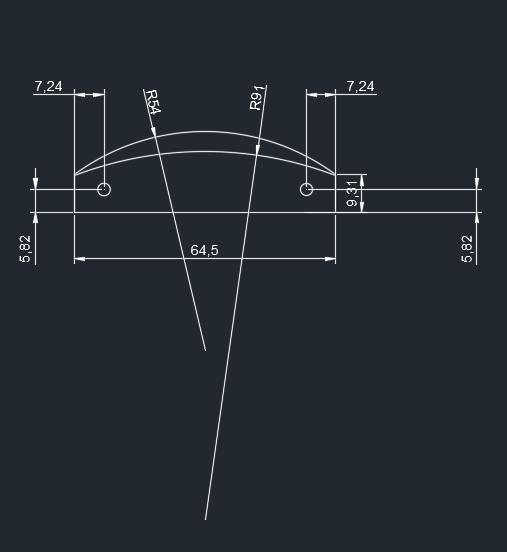
\includegraphics{figures/cad4_2}
	\caption{peça que conecta o suporte de protoboard e a base - 2}
	\label{fig:peca_juncao_2}
\end{figure}



\chapter{Modelagem 3D}
\label{att_fabricao_montagem_modelagem}

\begin{figure}[h]
	\centering
	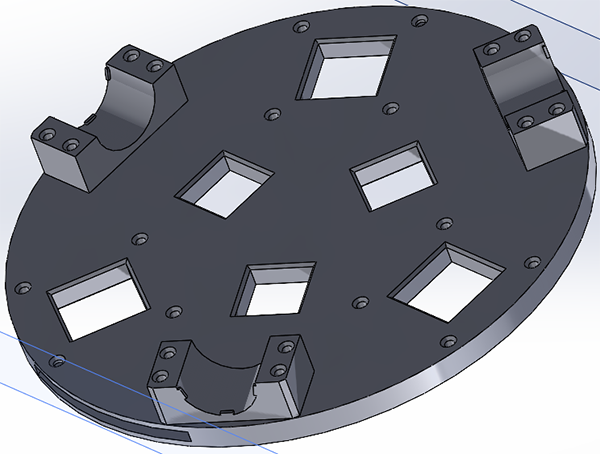
\includegraphics{figures/3d_1}
	\caption{Modelagem 3d da base do robô}
	\label{fig:base_robo_3d}
\end{figure}

\begin{figure}[h]
	\centering
	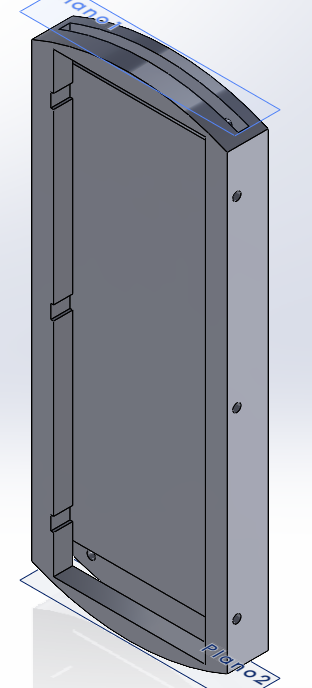
\includegraphics{figures/3d_2}
	\caption{Modelagem 3d do suporte do protoboard}
	\label{fig:suport_protoboard_3d}
\end{figure}

\begin{figure}[h]
	\centering
	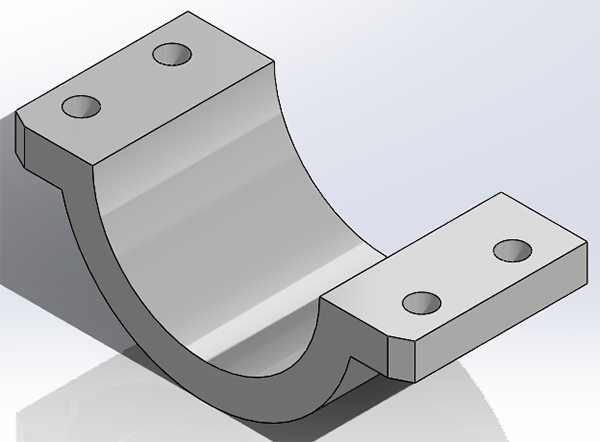
\includegraphics{figures/3d_3}
	\caption{Modelagem 3d dos mancais}
	\label{fig:mancais_3d}
\end{figure}

\begin{figure}[h]
	\centering
	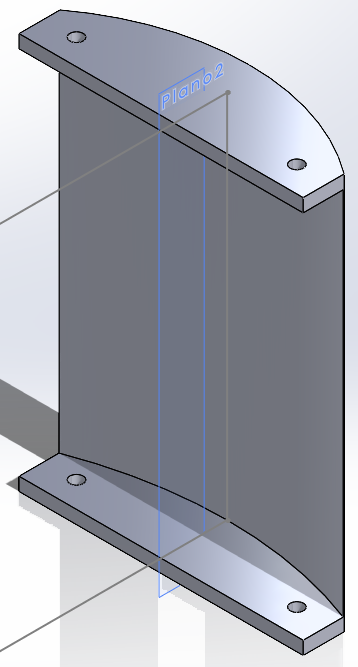
\includegraphics{figures/3d_4}
	\caption{Modelagem 3d peça de junção}
	\label{fig:peca_juncao_3d}
\end{figure}


\chapter{Impressão e montagem}
\label{att_fabricao_montagem_impressao}

\begin{figure}[h]
	\centering
	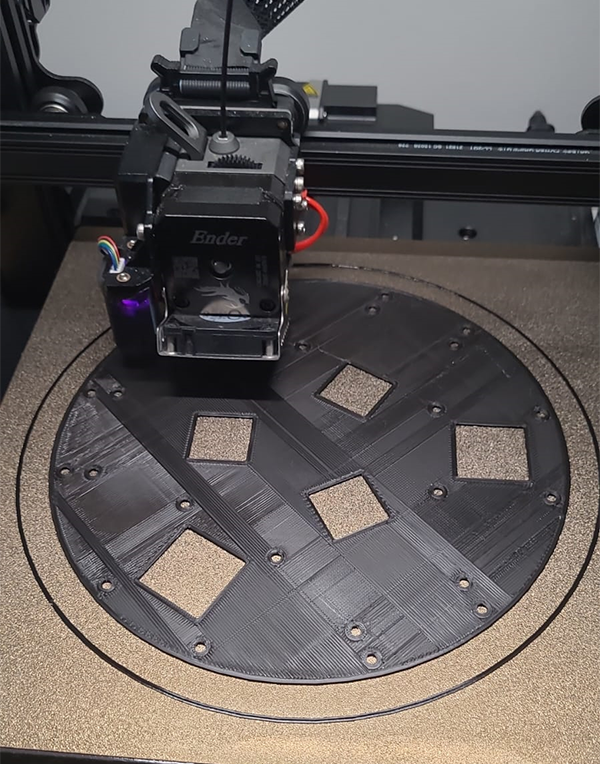
\includegraphics{figures/impressao}
	\caption{Impressão das peças}
	\label{fig:impressao}
\end{figure}

\begin{figure}[h]
	\centering
	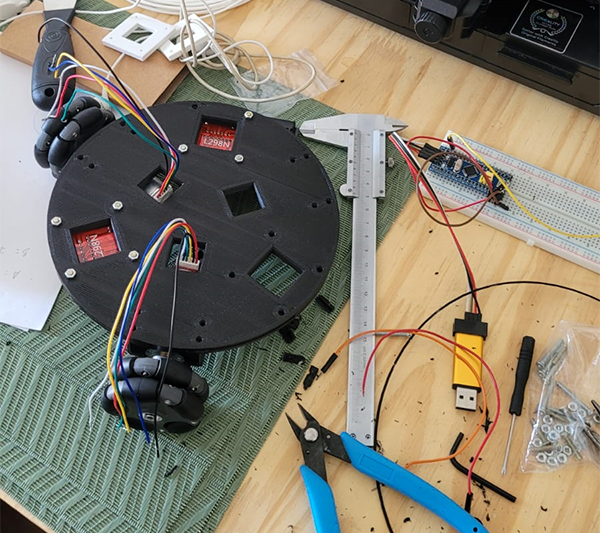
\includegraphics{figures/montagem_1}
	\caption{Montagem 1}
	\label{fig:montagem}
\end{figure}

\begin{figure}[h]
	\centering
	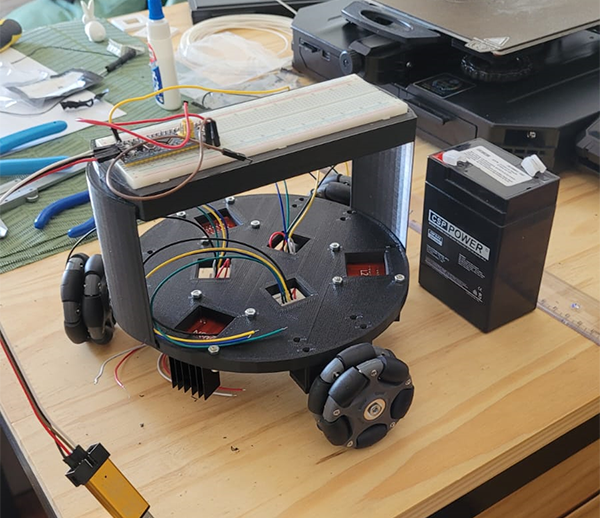
\includegraphics{figures/montagem_2}
	\caption{Montagem 2}
	\label{fig:montagem_2}
\end{figure}

\begin{figure}[h]
	\centering
	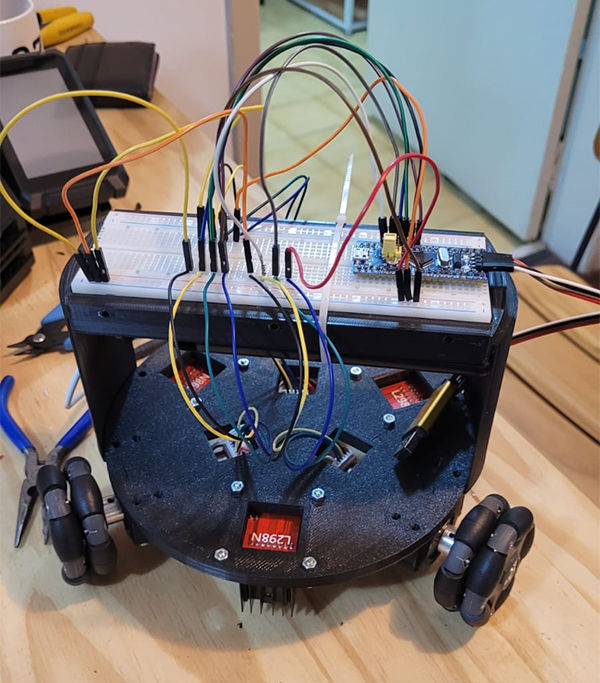
\includegraphics{figures/montagem_3}
	\caption{Montagem 3}
	\label{fig:montagem_3}
\end{figure}


\begin{figure}[h]
	\centering
	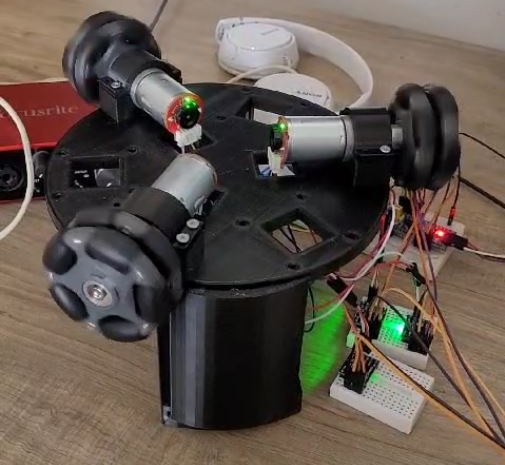
\includegraphics{figures/montagem_4}
	\caption{Testes dos motores}
	\label{fig:montagem_4}
\end{figure}


\section{Segurança}

\lipsum[1]

	
	

\chapter{Resultados e Discussão}

\lipsum[1]

	\phantompart

% ELEMENTOS PÓS-TEXTUAIS
\postextual

	% Referências bibliográficas

	
	
	\begin{apendicesenv}

% Imprime uma página indicando o início dos apêndices
% \partapendices




\chapter{Transcrição da matriz de cinemática em um bloco de código C \label{matriz_cinematica_c}}

\lstset{language=C}
\begin{lstlisting}
#include <math.h>
#define RADIUS_ROBOT 100
// mm, raio medido do centro ate o centro geometrico de cada roda
#define DEFAULT_SPEED 400 // mm/second   velocidade linear do robo.
#define RADIUS_WHEEL 34.5 //mm Raio da roda
#define PI 3.141592653589

float speedLinearToRpm(float speedLinear){
    float rpm = 60*speedLinear/(2*PI*RADIUS_WHEEL);
    return rpm;
}

void TransformationMatrixRpm(
	volatile long *w1, volatile long *w2, volatile long *w3,
	float linSpdPer, // percentagem da velocidade linear
	float dirAngle, float angSpd
){
	float linSpd_x, linSpd_y;
	linSpd_x = linSpdPer * DEFAULT_SPEED * cos(dirAngle * (PI/180));
	linSpd_y = linSpdPer * DEFAULT_SPEED * sin(dirAngle * (PI/180));

	float a1[3] = {0, -2.0/3,  RADIUS_ROBOT/3};
	float a2[3] = {1/sqrt(3), 1.0/3, RADIUS_ROBOT/3};
	float a3[3] = {-1/sqrt(3), 1.0/3, RADIUS_ROBOT/3};

	float spdLin1, spdLin2, spdLin3;
	spdLin1 = (a1[0] * linSpd_y) + (a1[1] * linSpd_x) + (a1[2] * angSpd);
	spdLin2 = (a2[0] * linSpd_y) + (a2[1] * linSpd_x) + (a2[2] * angSpd);
	spdLin3 = (a3[0] * linSpd_y) + (a3[1] * linSpd_x) + (a3[2] * angSpd);
	
	*w1 = speedLinearToRpm(spdLin1);
	*w2 = speedLinearToRpm(spdLin2);
	*w3 = speedLinearToRpm(spdLin3);	
}
\end{lstlisting}


\chapter{Transcrição da conversão de RGB para HSV em um bloco de código C \label{anx_rgb_to_hsv}}

\lstset{language=C}
\begin{lstlisting}
#include <stdio.h>
float maxOfThree(float a, float b, float c) {
	if ((a >= b) && (a >= c)) return a;
	else if ((b >= a) && (b >= c)) return b;
	else return c;
}
float minOfThree(float a, float b, float c) {
	if ((a <= b) && (a <= c)) return a;
	else if ((b <= a) && (b <= c)) return b;
	else return c;
}
void rgbToDirAngAndMag(int r, int g, int b, float *h, float *s) {
	float r_norm = r / 255.0, g_norm = g / 255.0, b_norm = b / 255.0;
	float cmax = maxOfThree(r_norm, g_norm, b_norm);
	float cmin = minOfThree(r_norm, g_norm, b_norm);
	float diff = cmax - cmin;
	if (cmax == cmin) {
		*h = 0;
	} else if (cmax == r_norm) {
		*h = fmod((60 * ((g_norm - b_norm) / diff) + 360), 360);
	} else if (cmax == g_norm) {
		*h = fmod((60 * ((b_norm - r_norm) / diff) + 120), 360);
	} else if (cmax == b_norm) {
		*h = fmod((60 * ((r_norm - g_norm) / diff) + 240), 360);
	}
	if (cmax == 0) {*s = 0;} else {*s = (diff / cmax) * 100;}
	*h = 360 - *h;
}
void main() {
	int r = 255, g = 0, b = 255; float h, s;
	rgbToDirAngAndMag(r, g, b, &h, &s);
	printf("Direction (Hue): %.2f\n", h); // res = 60
	printf("Magnitude (Saturation): %.2f\n", s); // res = 100
}
	
\end{lstlisting}
% 
\chapter{apendice 2}

\lipsum[1]


\end{apendicesenv}
	
	\bibliography{bibliography/bibliografia.bib}
	%\printbibliography


	% Glossário
	%%\glossary



	% Apêndices

	% Anexos
	% \begin{anexosenv}
	% \partanexos
	% \chapter{Medição de velocidade dos motores}
\label{att_medicao_motores}

\begin{figure}[ht]
	\centering
	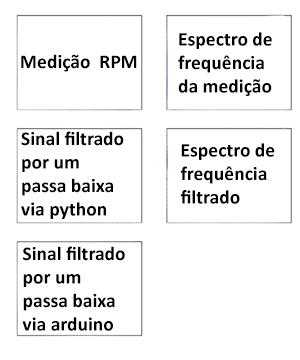
\includegraphics{figures/explicacao_quadros}
	\caption{Explicação de cada quadro nas figuras a seguir}
	\label{fig:explicacao_quadros}
\end{figure}


\begin{figure}[ht]
	\centering
	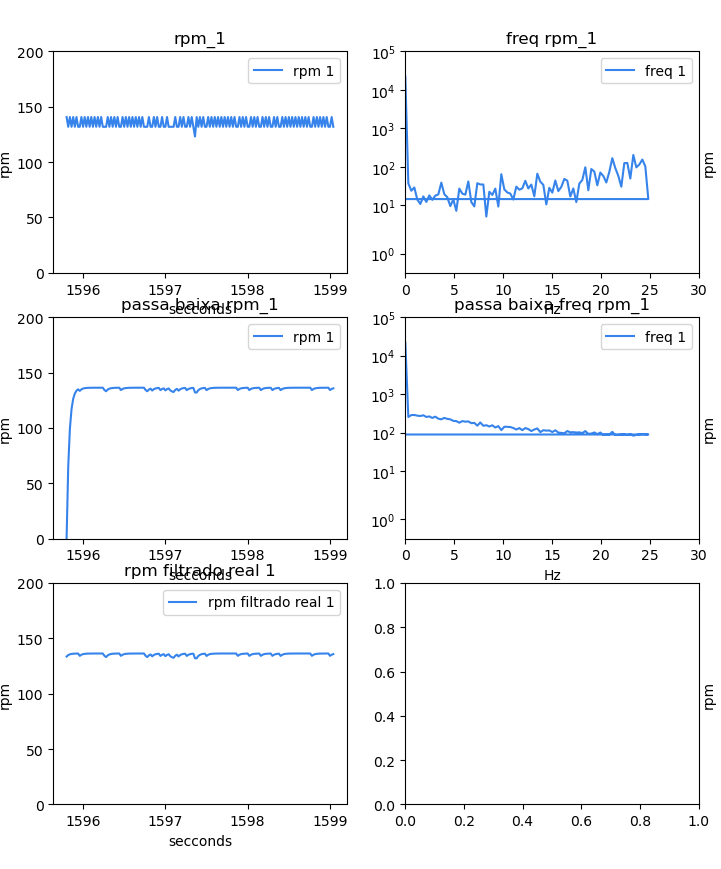
\includegraphics{figures/medidas_motor_1}
	\caption{Medidas Motor 1}
	\label{fig:medidas_motor_1}
\end{figure}

\begin{figure}[ht]
	\centering
	\includegraphics{figures/medidas_motor_2}
	\caption{Medidas Motor 2}
	\label{fig:medidas_motor_2}
\end{figure}


\begin{figure}[ht]
	\centering
	\includegraphics{figures/medidas_motor_3}
	\caption{Medidas Motor 3}
	\label{fig:medidas_motor_3}
\end{figure}




	% \end{anexosenv}
	

%---------------------------------------------------------------------
% INDICE REMISSIVO
%---------------------------------------------------------------------
\phantompart
\printindex


\end{document}
